% --------------------------------------------------------------
% This is all preamble stuff that you don't have to worry about.
% Head down to where it says "Start here"
% --------------------------------------------------------------
 
\documentclass[12pt]{article}
 

\usepackage[utf8]{inputenc}
\usepackage{intmacros}
\usepackage[margin=1in]{geometry} 
\usepackage{amsmath,amsthm,amssymb}
\usepackage[backend=biber, style=ieee, isbn=false,sortcites, maxbibnames=5, minbibnames=1]{biblatex}
\usepackage{hyperref}
\usepackage{xcolor}
\usepackage{amsmath}
\usepackage{graphicx}
\usepackage{caption,subcaption}
\captionsetup{labelsep = period} % Figure 2. Caption (rather than Figure 2: Caption)

\usepackage[]{hyperref}
\hypersetup{
	colorlinks   = true, %Colours links instead of ugly boxes
	urlcolor     = blue, %Colour for external hyperlinks
	linkcolor    = red, %Colour of internal links
	citecolor   = green %Colour of citations
}
\addbibresource{bibliography.bib}


\newenvironment{theorem}[2][Theorem]{\begin{trivlist}
\item[\hskip \labelsep {\bfseries #1}\hskip \labelsep {\bfseries #2.}]}{\end{trivlist}}
\newenvironment{lemma}[2][Lemma]{\begin{trivlist}
\item[\hskip \labelsep {\bfseries #1}\hskip \labelsep {\bfseries #2.}]}{\end{trivlist}}
\newenvironment{exercise}[2][Exercise]{\begin{trivlist}
\item[\hskip \labelsep {\bfseries #1}\hskip \labelsep {\bfseries #2.}]}{\end{trivlist}}
\newenvironment{reflection}[2][Reflection]{\begin{trivlist}
\item[\hskip \labelsep {\bfseries #1}\hskip \labelsep {\bfseries #2.}]}{\end{trivlist}}
\newenvironment{proposition}[2][Proposition]{\begin{trivlist}
\item[\hskip \labelsep {\bfseries #1}\hskip \labelsep {\bfseries #2.}]}{\end{trivlist}}
\newenvironment{corollary}[2][Corollary]{\begin{trivlist}
\item[\hskip \labelsep {\bfseries #1}\hskip \labelsep {\bfseries #2.}]}{\end{trivlist}}
 
\begin{document}
 
% --------------------------------------------------------------
%                         Start here
% --------------------------------------------------------------
 
%\renewcommand{\qedsymbol}{\filledbox}
 
\title{Assignment 1: EM for Categorical Data Advanced Signal Processing}%
\author{Daniel Barrejón Moreno} %if necessary, replace with your course title
 
\maketitle
 
\section{Problem formulation}
 
\noindent In this project we want to study a set of documents with a model following a mixture of categorical distributions. For a document $\x$ belonging to a set of documents $\X$, the marginal li,kelihood is expressed as follows
\begin{equation}\label{eq:marginal_x_given_z}
     p(\x|\bstheta) = \sum_{k=1}^{K}\pi_k\prod_{j=1}^{D}\Cat(x_j|\bstheta_k),
\end{equation}
where $K$ is the number of mixtures (in our case the topics), $D$ is the number of words that appear in a certain document and $\Cat(x_j|\bstheta_k)$ is the categorical distribution with $I$ categories and parameter $\bstheta_k$ which represents the probability that a certain category appears. Bear in mind that the model parameters are defined as $\bstheta = \{\bstheta_k, \bspi\}$. Since $\bstheta_k = (\theta_{k,1},\dots, \theta_{k,m}, \dots, \theta_{k,I})$ is a vector with the probabilities of topic $k$ probability, it must satisfy two constraints:
\begin{align}\label{eq:theta_constraint}
& 0 < \theta_{k,m} < 1\\
\text{and} \quad & \sum\limits_{m=1}^{I}\theta_{k,m} = 1.
\end{align}
\noindent The expression for the log li,kelihood of the observed data $\mathcal{D}$ looks li,ke this
\begin{equation}
\log p (\mathcal{D}|\bstheta) = \sum\limits_{n=1}^{N}\log p(\x|\bstheta) = \sum_{k=1}^{K}\pi_k\prod_{j=1}^{D}\Cat(x_j|\bstheta_k).
\end{equation}
However this function is hard to optimize due to the sum inside the $\log$. In order to solve this we introduce the latent variable $\mathcal{Z}$. The marginal distribution for the hidden variable $z_i$ is defined by the mixing coefficient of the mixture $\pi_k$ as follows
\begin{equation}
p(z_i=k) = \pi_k.
\end{equation}
Since $\bspi = \{\pi_1,\dots,\pi_K\}$ is a vector with the probabilities for the mixtures, certain restrictions must be satisfied:
\begin{align}\label{eq:pi_constraint}
& 0 < \pi_k < 1 \\
\text{and} \quad  & \sum\limits_{k=1}^{K} \pi_k = 1.
\end{align}
Now we need to find the expression for the complete data log li,kelihood $p(\mathcal{D},\mathcal{Z})$. First of all, the marginal of $z_i$ is given by
\begin{equation}\label{eq:marginal_z}
p(z_i|\bstheta) = \prod_{k=1}^{K}\pi_k^{\Ind \lbrace z_i=k \rbrace},
\end{equation}
where $\Ind(\cdot)$ is the indicator function. The probability density function for $x_i$ given $z_i$ is given by the following expression
\begin{equation}\label{eq:x_given_z}
p(\x_i|z_i,\bstheta) = \prod_{k=1}^{K}\prod_{j=1}^{D}\Cat(x_{ij}|\bstheta_k)^{\Ind \lbrace z_i=k \rbrace}.
\end{equation}
Since we are interested in the joint probability, applying Bayes' rule
\begin{equation}
p\left(\x_{i},z_{i}|\bstheta\right) = p\left(\x_{i}|z_{i},\bstheta\right) p(z_{i}|\bstheta)
\end{equation}
yields the resulting expression
\begin{equation}
p\left(\x_{i},z_{i}|\bstheta\right) = \prod\limits_{k=1}^{K}\left( \pi_{k} \prod \limits_{j=1}^{D} \text{Cat}(x_{ij}|\bstheta_{k}) \right)^{\Ind\lbrace z_{i}=k \rbrace}.
\end{equation}

\section{Complete data log likelihood $l_c(\bstheta) $}
\noindent Assuming that our observed data is independent and identically distributed (i.i.d) and taking natural logarithm we can find expression of the complete data log li,kelihood
\begin{align}
l_c(\bstheta) & = \log p(\mathcal{D},\mathcal{Z}|\bstheta) = \log \prod\limits_{n=1}^{N} p\left(\x_{i},z_{i}|\bstheta\right)\\
& = \sum_{i=1}^{N}\log p\left(\x_{i},z_{i}|\bstheta\right)\\
& = \sum_{i=1}^{N} \log \prod\limits_{k=1}^{K}\left( \pi_{k} \prod \limits_{j=1}^{D} \text{Cat}(x_{ij}|\bstheta_{k}) \right)^{\Ind\lbrace z_{i}=k \rbrace}\\
& = \sum_{i=1}^N\sum_{k=1}^K\Ind (z_i=k) \log\left( \pi_k\prod_{j=1}^D\Cat(x_{ij}|\bstheta_k)\right).
\end{align}
We can simplify the expression for the marginal of $\x_i$ as
\begin{align}\label{eq:marginal_x}
    p(\x_i) & = \prod_{j=1}^D\Cat(x_{ij}|\bstheta) = \prod_{j=1}^D\prod_{m=1}^I\theta_m^{\Ind \lbrace x_{i,j}=m \rbrace} = \prod_{m=1}^I\prod_{j=1}^D\theta_m^{\Ind \lbrace x_{i,j}=m \rbrace } \\
    & = \prod_{m=1}^I\theta_m^{\sum_{j=1}^D {\Ind \lbrace x_{i,j}=m \rbrace }} = \prod_{m=1}^I \theta_m^{\mu_{i,m}},
\end{align}
where we have defined a new metric $\mu_{i,m}$ that represents the number of times the word associated to the category $m$ appears at document $i$, \textit{i.e}.\ ,
\begin{equation}
    \mu_{i,m} = \sum_{j=1}^D {\Ind(x_{i,j}=m)}.
\end{equation}
Therefore, the final expression will be 
\begin{align}
    l_c(\bstheta) & = \sum_{i=1}^N\sum_{k=1}^K\Ind (z_i=k) \log\left( \pi_k\prod_{j=1}^D\Cat(x_{ij}|\bstheta_k)\right) \\
    & =  \sum_{i=1}^N\sum_{k=1}^K\Ind (z_i=k) \log \pi_k + \sum_{i=1}^N\sum_{k=1}^K\Ind (z_i=k) \log \prod_{m=1}^I \theta_{k,m}^{\mu_{i,m}}\\
    & = \sum_{i=1}^N\sum_{k=1}^K\Ind (z_i=k) \log \pi_k + \sum_{i=1}^N\sum_{k=1}^K\Ind (z_i=k) \sum_{m=1}^I \mu_{i,m}\log \theta_{k,m} \label{eq:log_li,ke}.
\end{align}
    
   
\section{ML Inference}

\noindent In order to solve the maximum li,kelihood problem, we define an auxiliary function $Q$ which will be the expected complete data log li,kelihood over the hidden variable $\mathcal{Z}$. This function $Q$ will be evaluated in the E-step and maximized for the model parameters $\bstheta$ to update the model parameters in each iteration of the algorithm.
\subsection{E-step: $Q(\bstheta^t, \bstheta^{t-1})$ for ML inference}

Taking the expectation with respect to the latent variables $z$ we get the following expected complete data log-li,kelihood.
\begin{align}
    Q(\bstheta^t, \bstheta^{t-1}) & = \expectation_Z\{l_c(\bstheta)|\mathcal{D},\bstheta^{t-1}\}  \\
    & = \sum_{i=1}^N\sum_{k=1}^K\expectation_Z\{\Ind (z_i=k)\} \log \pi_k + \sum_{i=1}^N\sum_{k=1}^K\expectation_Z\{\Ind(z_i=k)\} \sum_{m=1}^I \mu_{i,m}\log \theta_{k,m}\\
    & = \sum_{i=1}^N\sum_{k=1}^K r_{i,k}\log \pi_k + \sum_{i=1}^N\sum_{k=1}^K r_{i,k}\sum_{m=1}^I \mu_{i,m}\log \theta_{k,m} \label{eq:Q_function},
\end{align}
where we have defined the metric $r_{i,k} \triangleq p(z_i = k | \x_i,\bstheta^{t-1})$ \cite{murphy2012machine} as the responsibility that mixture $k$, \textit{i.e.\ } topic $k$, takes at explaining the document $\x_i$. It is defined as follows
\begin{align}\label{eq:r_i,k}
	r_{i,k} & = \expectation_Z\{ \Ind(z_i=k) \} = p(z_i = k|\x_i,\bstheta^{t-1}) \\
	& = \frac{p(z_i=k,\x_i|\bstheta^{t-1})}{p(\x_i|\bstheta^{t-1})} = \frac{p(z_i=k,\x_i|\bstheta^{t-1})}{\sum \limits_{k\prime}^{K}p(z_i=k\prime,\x_i|\bstheta^{t-1})}\\
	& = \frac{\pi_k p(\x_i|\bstheta_k)}{\sum \limits_{k\prime}^K \pi_{k\prime} p(\x_i|\bstheta_{k\prime})}  =	\frac{\pi_k\prod_{j=1}^{D}\Cat(x_{i,j}|\bstheta_k)}{\sum \limits_{k\prime}^{K} \pi_{k\prime} \prod \limits_{j=1}^{D}\Cat(x_{i,j}|\bstheta_k\prime)}.
\end{align}
This quantity must satisfy the following constrains, given that z it is a probability
\begin{align}\label{eq:ri,k_constriant}
& 0 \leq r_{i,k} \leq 1, \\
\text{and} \quad & \sum \limits_{k=1}^{K} r_{i,k} = 1.
\end{align}

\subsubsection{Arithmetic underflow solved by log-sum-exp trick}

In our problem we have $I$ categories which correspond to the words from a dictionary. When we perform the product in Equation \ref{eq:r_i,k} we obtain really small values that cannot be represented by the computer. This problem is known as \textbf{arithmetic underflow}. However, in order to maintain the range in probability if categories $\theta_{k,m}$ that influence the value of $r_{i,k}$ we use the \textbf{log-sum-exp trick} \cite{logsumexp}.

\noindent Taking the logarithm from Equation \ref{eq:r_i,k} and using Equation \ref{eq:marginal_x} for $p(\x_i|\bstheta_k)$ we obtain the following expression
\begin{align}\label{eq:log_rik}
\log r_{i,k} & = \log \pi_k\prod_{j=1}^{D}\Cat(x_{i,j}|\bstheta_k) - \log \sum \limits_{k\prime=1}^{K} \pi_{k\prime} \prod \limits_{j=1}^{D}\Cat(x_{i,j}|\bstheta_k\prime)\\
& = \log \pi_k + \sum\limits_{m=1}^{I}\mu_{i,m}\log\theta_{k,m} - \log \sum \limits_{k\prime=1}^{K} \pi_{k\prime} \prod \limits_{m=1}^{I} \theta_{k\prime,m}^{\mu_{i,m}}.
\end{align}
The log-sum-exp trick will be applied on the last term from the above equation. The trick states that
\begin{equation}
\log \sum _ { v = 1 } ^ { V } e ^ { g _ { v } } = a + \log \sum _ { v = 1 } ^ { V } e ^ { g _ { v } - a },
\end{equation}
where $a = \max_{\substack{v}} g_v$ and $g_v$ is defined as 
\begin{equation}
g_v = \log \pi_{k\prime} \prod \limits_{m=1}^{I} \theta_{k\prime,m}^{\mu_{i,m}} = \log \pi_{k\prime} + \sum\limits_{m=1}^{I}\mu_{i,m} \log \theta_{k\prime,m}
\end{equation}
Once $\log r_{i,k}$ from Equation \ref{eq:log_rik} is known, we can find $r_{i,k}$ with an exponential. With this trick we do not loose any information by forcing values assigned to be 0 by the computer using clipping and we also increase computational speed. 

\subsection{M-step for ML inference}

\noindent Now we need to find the closed-form formulas to update the model parameters $\bstheta = \{\bstheta_k, \bspi\}$. Since we must tackle a maximization problem with constraints we will apply Lagrange Multipliers to solve equation
\begin{equation}
\boldsymbol { \theta } ^ { t } = \underset { \boldsymbol { \theta } } { \operatorname { argmax } } Q \left( \boldsymbol { \theta } , \boldsymbol { \theta } ^ { t - 1 } \right).
\end{equation}

\subsubsection{Maximization of $\pi_k$}

\noindent Using the constraints on $\pi$ from Equations \ref{eq:pi_constraint} we propose as Lagrangian the function
\begin{equation}\label{eq:lagrange_pi,k}
L\left( Q(\pi_{k}),\lambda \right) = Q(\pi_{k}) + \lambda \left( \sum \limits_{k=1}^{K} \pi_{k} - 1 \right),
\end{equation}
which will be optimized in this way
\begin{equation}\label{minmax_lagrange_pi,k}
\min_{\substack{\lambda}}\max_{\substack{\pi_{k}}} \lbrace L\left( Q(\pi_{k}),\lambda \right) \rbrace.
\end{equation}

\noindent  First, we take the derivative of Equation \ref{eq:lagrange_pi,k} w.r.t $\pi_{k}$ and equate it to 0, which yields
\begin{align}\label{deriv_pi,k}
& \dfrac{\partial L}{\partial \pi_{k}} = 0 = \sum \limits_{i=1}^{N} \dfrac{r_{i,k}}{\pi_{k}} - \lambda, \\
& \pi_{k} = \dfrac{1}{\lambda} \sum \limits_{i=1}^{N} r_{i,k} \label{eq:pi_k_deriv}.
\end{align}
Now, we take the derivate w.r.t $\lambda$ which yields
\begin{align}
& \dfrac{\partial L}{\partial \lambda} = \sum \limits_{k=1}^{K} \pi_{k} - 1  = 0 ,\\
& \sum \limits_{k=1}^{K} \pi_{k} = 1.
\end{align}
If we sum over $k$ at both sides of Equation \ref{eq:pi_k_deriv}
\begin{align}
& \sum \limits_{k=1}^{K}\pi_{k} = \sum \limits_{k=1}^{K} \dfrac{1}{\lambda} \sum \limits_{i=1}^{N} r_{i,k}\\
& 1 = \dfrac{1}{\lambda} \sum \limits_{i=1}^{N}\sum \limits_{k=1}^{K}r_{i,k},
\end{align}
and using the constraints on $r_{i,k}$ from Equations \ref{eq:ri,k_constriant} we get the value of $\lambda$
\begin{align}
& 1 = \dfrac{1}{\lambda} \sum \limits_{i=1}^{N}1.\\
& \lambda = N.
\end{align}
Knowing the value of $\lambda$ the estimated value of $\hat{\pi}_{k}$ can be expressed as follows
\begin{align}\label{eq:pi_k}
& \hat{\pi}_{k} = \dfrac{1}{N} \sum \limits_{i=1}^{N} r_{i,k}s = \frac{N_k}{N},
\end{align}
where 
\begin{equation}\label{eq:N_k}
N_k = \sum_{i=1}^N r_{i,k}.
\end{equation}
This result is actually intuitive since $N_k$ represents the 'weight' of topic $k$ at explaining the documents, and therefore $\pi_k$ is just the percentage of topic $k$ at explaining the data.

\subsubsection{Maximization of $\bstheta_k$}

\noindent We follow a similar approach. Now, using the constraints on $\bstheta_k$ from Equations \ref{eq:theta_constraint} we propose as Lagrangian the following function
\begin{equation}\label{eq:lagrange_thetakm}
L\left( Q(\theta_{k,m}),\lambda \right) = Q(\theta_{k,m}) + \lambda \left( \sum \limits_{m=1}^{I} \theta_{k,m} - 1 \right),
\end{equation}
which will be optimized as a min-max problem
\begin{equation}\label{minmax_lagrange_thetakm}
\min_{\substack{\lambda}} \max_{\substack{\theta_{km}}} \lbrace L\left( Q(\theta_{km}),\lambda \right) \rbrace.
\end{equation}
Firstly, we take the derivative of Equation \ref{eq:lagrange_thetakm} w.r.t $\theta_{k,m}$ and equate it to 0, which yields
\begin{align}\label{deriv_thetakm}
& \dfrac{\partial L}{\partial \theta_{k,m}} = \sum \limits_{i=1}^{N} \dfrac{r_{i,k}\mu_{i,m}}{\theta_{k,m}} - \lambda = 0 , \\
& \theta_{k,m} = \dfrac{1}{\lambda} \sum \limits_{i=1}^{N} r_{i,k}\mu_{i,m} \label{eq:theta_k_deriv}.
\end{align}
Secondly, we take the derivative w.r.t $\lambda$, which yields
\begin{align}
& \dfrac{\partial L}{\partial \lambda} = \sum \limits_{m=1}^{I} \theta_{k,m} - 1 = 0,\\
& \sum \limits_{m=1}^{I} \theta_{k,m} = 1.
\end{align}
If now we sum over $I$ at both sides of Equation \ref{eq:theta_k_deriv}, the value of $\lambda$ is obtained
\begin{align}
& \sum \limits_{m=1}^{I}\theta_{k,m} = \sum \limits_{m=1}^{I} \dfrac{1}{\lambda} \sum \limits_{i=1}^{N} r_{i,k}\mu_{i,m}\\
& 1 = \dfrac{1}{\lambda} \sum \limits_{i=1}^{N}\sum \limits_{m=1}^{I}r_{i,k}\mu_{i,m},\\
& \lambda = \sum \limits_{i=1}^{N}\sum \limits_{m=1}^{I}r_{i,k}\mu_{i,m}.
\end{align}
Using the value of $\lambda$ in Equation \ref{eq:theta_k_deriv}, $\theta_{k,m}$ is obtained
\begin{equation}\label{eq:theta_km}
\hat{\theta}_{k,m} = \dfrac{\sum \limits_{i=1}^{N} r_{i,k}\mu_{i,m}}{\sum \limits_{i=1}^{N}\sum \limits_{m=1}^{I}r_{i,k}\mu_{i,m}}.
\end{equation}
Again, the result is quite intuitive. $\theta_{k,m}$ is just the average of the category $m$ weighted by the responsibility $r_{i,k}$.

\section{MAP inference}

Maximum li,kelihood estimations is an estimation that tends to overfit \cite{murphy2012machine}. A solution to such problem is applying maximum a posteriori estimation (MAP). In this case, we do not only consider the li,kelihood, but also some prior information on the model parameters $\bstheta$. From Bayes' rule we know that
\begin{equation}
p(\boldsymbol{\theta}|\mathcal{D},\mathcal{Z}) \varpropto p(\mathcal{D},\mathcal{Z}|\boldsymbol{\theta})p(\boldsymbol{\theta}).
\end{equation}
If we take logarithms at both sides of the equation we get
\begin{equation}
\log p(\boldsymbol{\theta}|\mathcal{D},\mathcal{Z}) \varpropto \log p(\mathcal{D},\mathcal{Z}|\boldsymbol{\theta}) + \log p(\boldsymbol{\theta}) .
\end{equation}
Notice that the first term is just the complete data log li,kelihood from Equation \ref{eq:log_li,ke} and the second term corresponds to the prior information. The goal now is to define some prior over the model parameters $\bstheta$ and use it on the function $Q$ from Equation \ref{eq:Q_function} to work with the posterior instead of the li,kelihood. Afterwards, we need to reformulate Equation \ref{eq:pi_k} and \ref{eq:theta_km} for $\pi_k$ and $\theta_{k,m}$ to take into account the priors.\\

\subsection{E-step: $Q(\bstheta^t, \bstheta^{t-1})$ for MAP inference}
\noindent From \cite{notesArtes} and \cite{murphy2012machine} we know it is natural that the prior on the mixture weights $\pi$ and the category probabilities $\bstheta_k$ follow a Dirichlet distribution, \textit{i.e.\ },
\begin{align}\label{priors}
& \bspi \sim \text{Dir}(\bsbeta), \quad \text{s.t.} \quad  p(\bspi |\bsbeta) = \dfrac{1}{\text{B}(\boldsymbol{\beta})} \prod \limits_{k=1}^{K} \pi_{k}^{\beta_{k}-1}, \\
& \bstheta_{k} \sim \text{Dir}(\bsalpha), \quad \text{s.t.} \quad p(\bstheta_{k}|\bsalpha) = \dfrac{1}{\text{B}(\boldsymbol{\alpha})} \prod \limits_{m=1}^{I} \theta_{k,m}^{\alpha_{m}-1},
\end{align}
where the function B(·) stands for the Beta function, and the parameters $\boldsymbol{\beta}$ and $\boldsymbol{\alpha}$ are the parameters or hyperpriors of the Dirichlet distributions for $\bspi$ and $\bstheta_{k}$ respectively. \\


\noindent The expression for the new $Q$ function is as follows
\begin{equation}\label{eq:Q_map_deriv}
Q(\bstheta^t, \bstheta^{t-1}) = \sum_{i=1}^N\sum_{k=1}^K r_{i,k}\log \pi_k + \sum_{i=1}^N\sum_{k=1}^K r_{i,k}\sum_{m=1}^I \mu_{i,m}\log \theta_{k,m} + \log p(\bspi|\bsbeta) + \sum\limits_{k=1}^{K}\log p(\bstheta_k|\bsalpha),
\end{equation}
where $r_{i,k}$ remains the same. Taking logarithm on the probability of the priors we get
\begin{align}
& \log p(\bspi|\bsbeta) = \log \left (\dfrac{1}{\text{B}(\bsbeta)} \prod \limits_{k=1}^{K} \pi_{k}^{\beta_{k}-1} \right )= \log \dfrac{1}{\text{B}(\bsbeta)} + \sum \limits_{k=1}^{K}(\beta_{k}-1)\text{log}(\pi_{k}),\\
& \log p(\bstheta_{k}|\bsalpha) = \log \left(\dfrac{1}{\text{B}(\bsalpha)} \prod \limits_{m=1}^{I} \theta_{k,m}^{\alpha_{m}-1}\right) = \log \dfrac{1}{\text{B}(\bsalpha)} +  \sum \limits_{m=1}^{I}(\alpha_{m}-1)\log (\theta_{k,m}).
\end{align}
\noindent Using these results in Equation \ref{eq:Q_map_deriv} we get the expression for $Q(\bstheta,\bstheta^{t-1})$ using MAP estimation
\begin{align}\label{eq:Q_map}
Q(\bstheta^t, \bstheta^{t-1})& = \sum_{i=1}^N\sum_{k=1}^K r_{i,k}\log \pi_k + \sum_{i=1}^N\sum_{k=1}^K r_{i,k}\sum_{m=1}^I \mu_{i,m}\log \theta_{k,m} \\
& + \log \left(\dfrac{1}{\text{B}(\bsbeta)}\right) + \sum \limits_{k=1}^{K}(\beta_{k}-1)\text{log}(\pi_{k})\\
& + \sum\limits_{k=1}^{K} \log \dfrac{1}{\text{B}(\bsalpha)} +  \sum\limits_{k=1}^{K}\sum \limits_{m=1}^{I}(\alpha_{m}-1)\log (\theta_{k,m}).
\end{align}
Notice that $\text{B}(\bsalpha)$ can be decomposed as $$
\mathrm { B } ( \boldsymbol { \alpha } ) = \frac { \prod _ { i = 1 } ^ { K } \Gamma \left( \alpha _ { i } \right) } { \Gamma \left( \sum _ { i = 1 } ^ { K } \alpha _ { i } \right) },
$$
where $\Gamma(\cdot)$ is the Gamma function. The same applies for $\text{B}(\bsbeta)$


\subsection{M step for MAP inference}

\noindent We will follow the same procedure as for the ML case; but now we must use function \ref{eq:Q_map} instead to take into account the priors.

\subsubsection{MAP estimation of $\pi_{k}$}

\noindent Again, we have the same maximization problem and hence we propose the same Lagrangian as in Equation \ref{eq:lagrange_pi,k} and we use the same constraints on $\pi_k$
\begin{equation}
L\left( Q(\pi_{k}),\lambda \right) = Q(\pi_{k}) + \lambda \left( \sum \limits_{k=1}^{K} \pi_{k} - 1 \right).
\end{equation}
Again, we derivative Equation \ref{eq:Q_map} w.r.t $\pi_{k}$ and equate it to 0
\begin{align}
& \dfrac{\partial L}{\partial \pi_{k}} =  \sum \limits_{i=1}^{N} \dfrac{r_{i,k}}{\pi_{k}} + \dfrac{\beta_{k}-1}{\pi_k} - \lambda = 0 ,\\
& \pi_{k} = \dfrac{1}{\lambda} \left( \sum \limits_{i=1}^{N} r_{i,k} + \beta_{k} - 1\right)\label{eq:deriv_pi,k_MAP}.
\end{align}
Now we derivate w.r.t $\lambda$
\begin{align}
& \dfrac{\partial L}{\partial \lambda} = \sum \limits_{k=1}^{K} \pi_{k} - 1 = 0 , \\
& \sum \limits_{k=1}^{K} \pi_{k} = 1.
\end{align}
Summing over $K$ at both sides of Equation \ref{eq:deriv_pi,k_MAP}
\begin{align}
& \sum \limits_{k=1}^{K}\pi_{k} = \sum \limits_{k=1}^{K} \dfrac{1}{\lambda} \left( \sum \limits_{i=1}^{N} r_{i,k} + \beta_{k} - 1\right)\\
& 1 = \dfrac{1}{\lambda} \sum \limits_{k=1}^{K} \sum \limits_{i=1}^{N} r_{i,k} + \dfrac{1}{\lambda} \sum \limits_{k=1}^{K} \beta_{k} - \dfrac{1}{\lambda} \sum \limits_{k=1}^{K} 1,
\end{align}
we get the value of $\lambda$
\begin{equation}
\lambda = N + \sum \limits_{k=1}^{K} \beta_{k} - K.
\end{equation}
Once $\lambda$ is known the estimated value of $\pi_{k}$ is as follows
\begin{equation}\label{eq:pi_map}
\hat{\pi}_{k} = \dfrac{\sum \limits_{i=1}^{N} r_{i,k} + \beta_{k} - 1}{N + \sum \limits_{k=1}^{K} \beta_{k} - K}.
\end{equation}

\subsubsection{MAP estimation of $\theta_{k,m}$}

\noindent For the estimation of $\theta_{k,m}$ we use the same Lagrangian from Equation \ref{eq:lagrange_thetakm} and the same restrictions from \ref{eq:theta_constraint} 
\begin{equation}
L\left( Q(\theta_{k,m}),\lambda \right) = Q(\theta_{k,m}) + \lambda \left( \sum \limits_{m=1}^{I} \theta_{k,m} - 1 \right).
\end{equation}
As before, we first derivate w.r.t $\theta_{k,m}$, which yields
\begin{align}
& \dfrac{\partial L}{\partial \theta_{k,m}} = \sum \limits_{i=1}^{N} \dfrac{r_{i,k}\mu_{im}}{\theta_{k,m}} + \dfrac{\alpha_m-1}{\theta_{km}} - \lambda = 0, \\
& \theta_{k,m} = \dfrac{1}{\lambda} \left( \sum \limits_{i=1}^{N} r_{i,k}\mu_{i,m} +\alpha_m - 1\right) \label{eq:deriv_thetakm_MAP}.
\end{align}
And later with respect to $\lambda$
\begin{align}
& \dfrac{\partial L}{\partial \lambda} = 0 = \sum \limits_{m=1}^{I} \theta_{k,m} - 1,\\
& \sum \limits_{m=1}^{I} \theta_{k,m} = 1.
\end{align}
Summing at both sides over $I$ Equation \ref{eq:deriv_thetakm_MAP} we can obtain the value of $\lambda$
\begin{align}
& \sum \limits_{m=1}^{I}\theta_{k,m} = \sum \limits_{m=1}^{I} \dfrac{1}{\lambda} \left( \sum \limits_{i=1}^{N} r_{i,k}\mu_{i,m} + \alpha_m - 1 \right)\\
& 1 = \dfrac{1}{\lambda} \sum \limits_{m=1}^{I} \left( \sum \limits_{i=1}^{N} \dfrac{r_{i,k}\mu_{i,m}}{\theta_{k,m}} + \dfrac{\alpha_m}{\theta_{k,m}} - 1 \right),\\
& \lambda = \sum \limits_{m=1}^{I} \sum \limits_{i=1}^{N} r_{i,k}\mu_{i,m} + \sum \limits_{m=1}^{I} \alpha_m - \sum \limits_{m=1}^{I} 1,\\
& \lambda = \sum \limits_{m=1}^{I} \sum \limits_{i=1}^{N} r_{i,k}\mu_{i,m} + \sum \limits_{m=1}^{I} \alpha_m - I.
\end{align}
And with that value of $\lambda$ the estimated value of $\theta_{k,m}$ is
\begin{equation}\label{eq:theta_map}
\hat{\theta}_{k,m} = \dfrac{\sum \limits_{i=1}^{N} r_{i,k}\mu_{im} +\alpha_m - 1}{\sum \limits_{m=1}^{I} \sum \limits_{i=1}^{N} r_{i,k}\mu_{i,m} + \sum \limits_{m=1}^{I} \alpha_m - I}.
\end{equation}

\section{Experiments}

The experiments have been divided into two sets: a set of experiment using ML estimation and another set using MAP estimation. For both sets of experiments the maximum number of iterations of the EM algorithm has been set to 100 iterations, the tolerance value has been set to $10^{-3}$ and a total of 5 different initializations have been done.

In order to assess the performance of the algorithm, for the two approaches the log-likelihood will be shown, as well as the responsibilities for each document $r_{i,k}$. In order to obtain a better visualization of the results, a word cloud for the different found topic will be shown, so that the most common words for each topic can be displayed and they could be associated to a certain abstract theme. 

\subsection{ML Experiments}

From the setup described above, it can be seen from Figure \ref{fig:Q_ML} that the log-likelihood is always increasing, and it actually converges reasonably fast. As it is known from the literature, the EM algorithm is quite likely to achieve a good solution rather fast, and then it tends to continue increasing in a plateau-fashion way.

% Q ML Figures
\begin{figure}[h]
	\centering
	\begin{subfigure}{0.4\textwidth}
		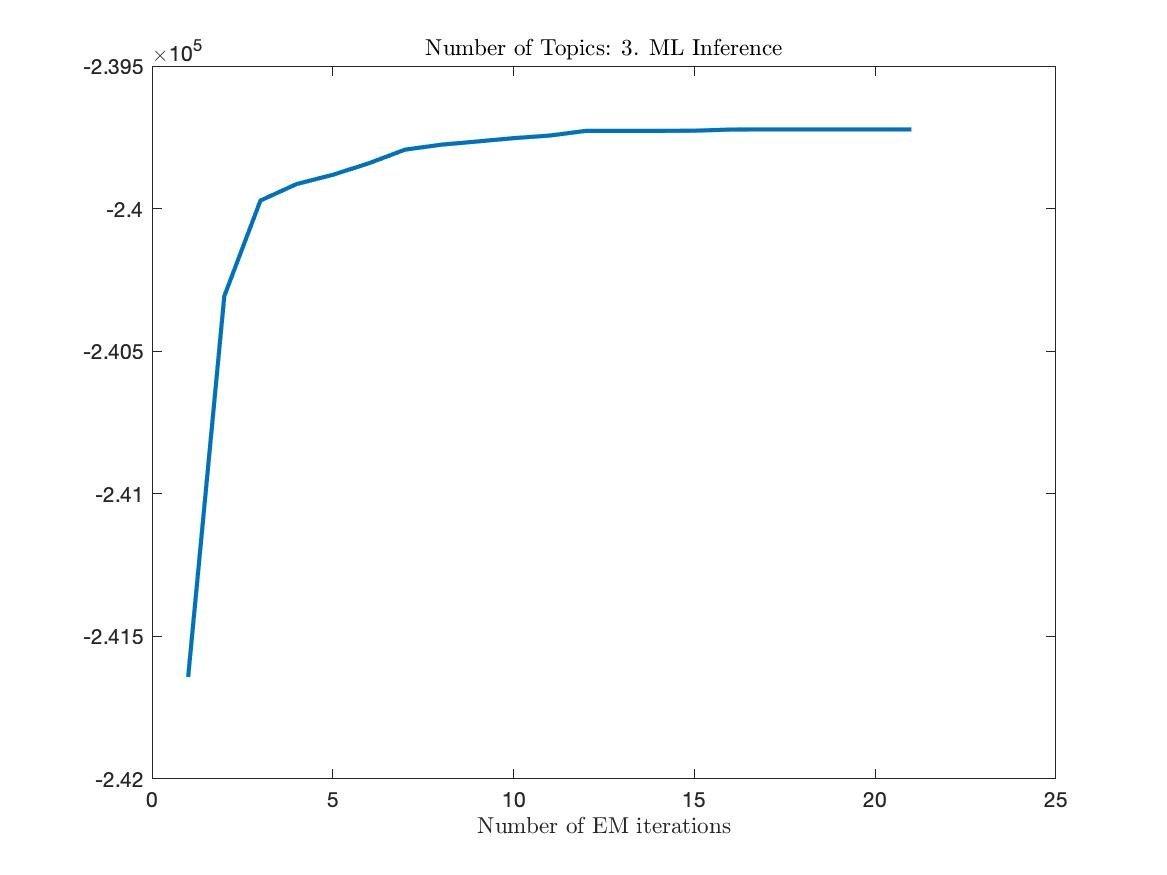
\includegraphics[width=\textwidth]{images/ML/Q_ml_3_topics.jpg}
		\caption{}
		\label{fig:Q_ML_3}
	\end{subfigure}
	~	
	\begin{subfigure}{0.4\textwidth}
		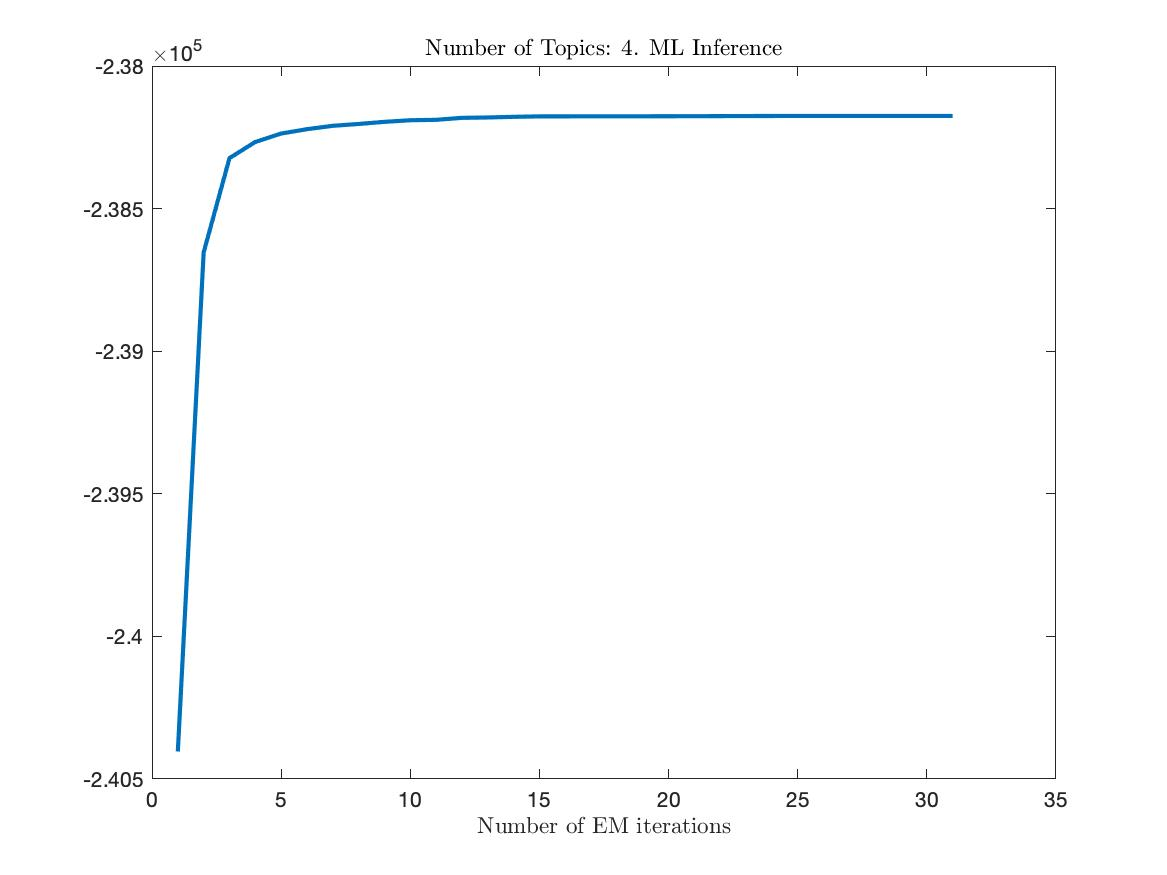
\includegraphics[width=\textwidth]{images/ML/Q_ml_4_topics.jpg}
		\caption{}
		\label{fig:Q_ML_4}
	\end{subfigure}
	\caption{The log-likelihood is increasing for both $K=3$ in Figure \ref{fig:Q_ML_3} and for $K=4$ in Figure \ref{fig:Q_ML_4}}
	\label{fig:Q_ML}
\end{figure}
In Figure \ref{fig:R_ML} it can bee seen the probabilities for each document for belonging to a certain topic. This result is obtained from the matrix of $r_{i,k}$. Although it is clear that each document is associated to a certain topic, still the results is quite scattered. With detailed observation it can be seen that there are some segments of following documents that might belong to a same topic, and hence we could differentiate different segments of documents.

% R ML Figures
\begin{figure}[h]
	\centering
	\begin{subfigure}{0.4\textwidth}
		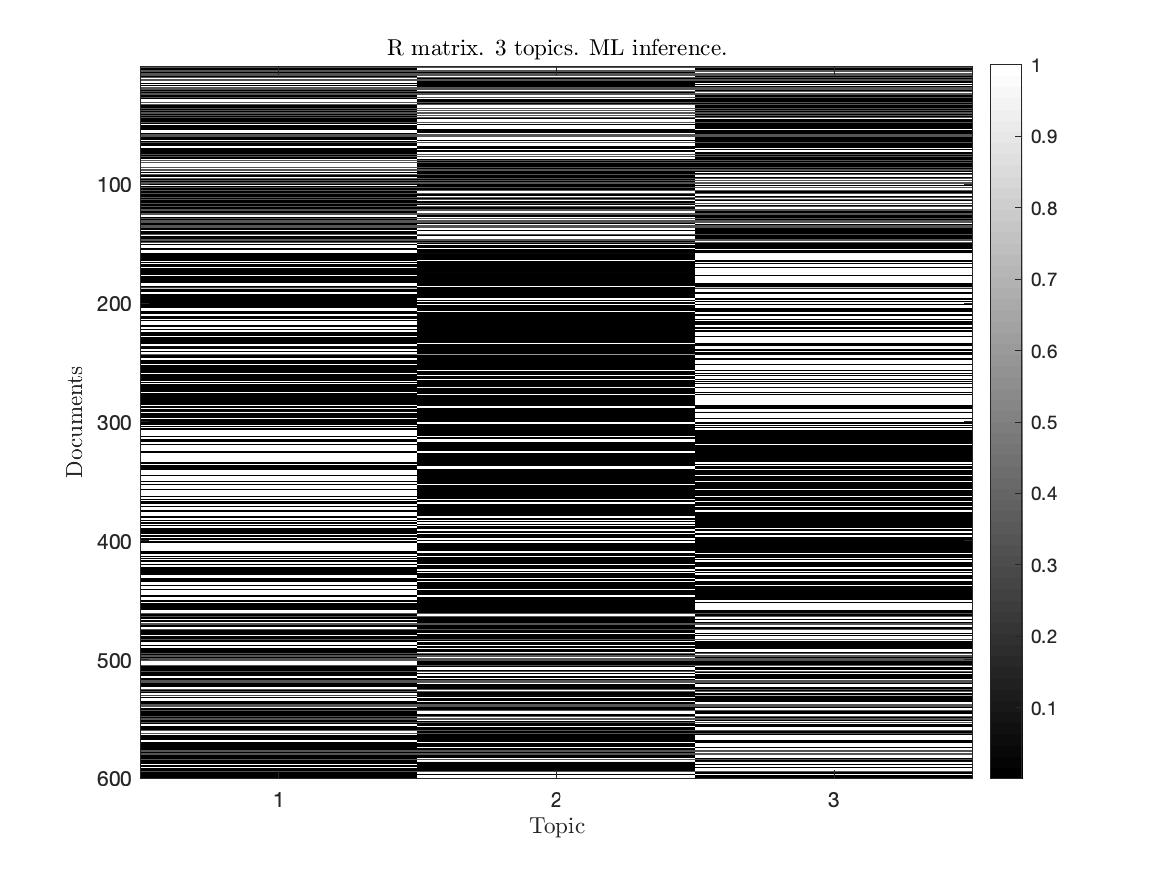
\includegraphics[width=\textwidth]{images/ML/R_ml_3_topics.jpg}
		\caption{}
		\label{fig:R_ML_3}
	\end{subfigure}
	~	
	\begin{subfigure}{0.4\textwidth}
		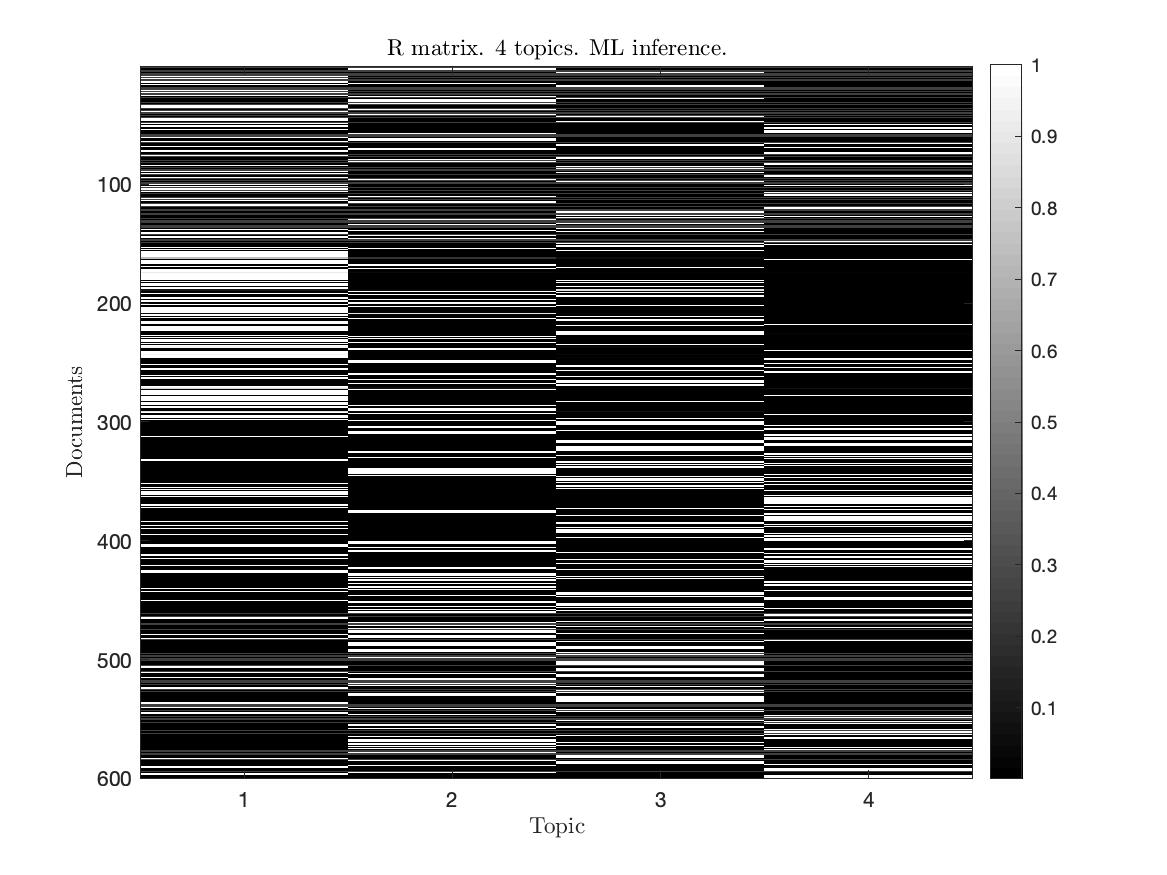
\includegraphics[width=\textwidth]{images/ML/R_ml_4_topics.jpg}
		\caption{}
		\label{fig:R_ML_4}
	\end{subfigure}
	\caption{Figures \ref{fig:R_ML_3} and \ref{fig:R_ML_4} show the probability of a certain document to be in a specific topic. As it can be seen, the result is quite scattered. This will be solved with the prior information in the MAP estimation.}
	\label{fig:R_ML}
\end{figure}


\subsection{MAP Experiments}

From Figure \ref{fig:R_ML} it could be seen that with the ML inference approach it is not possible to achieve the desired result of segments of documents with the same topic. To obtain this we need to incorporate some prior information about how we believe the topics and the categories of each document are distributed. To do so, we show three different experiments. For all of them the hyperparameter $\bsbeta$ has been set as $\bsbeta = 2\I_{Kx1}$ and $\bsalpha$ was set to 
$\bsalpha = 1.1\I_{Ix1}$, $\bsalpha = 5\I_{Ix1}$ and finally $\bsalpha = 2\I_{Ix1}$. For smaller values of $\bsalpha$ and $\bsbeta$ in the order of 0.5 the algorithm breaks since the results for Equations \ref{eq:theta_map} and \ref{eq:pi_map} are close to 0 and therefore the evaluation of the posterior in Equation \ref{eq:Q_map} returns complex values.

\subsubsection{Experiment 1: $\bsalpha = 1.1\I_{Ix1}$} 

In this case, choosing $\bsalpha = 1.1\I_{Ix1}$ is almost the same as choosing it uniformly, meaning that the prior probability for each different category of the categorical distribution is the same. As it was expected, the results is quite similar to the result obtained with the ML approach. The log-likelihood and the $r_{i,k}$ results are depicted in Figure \ref{fig:MAP_1.1} for value $K=3$.

% ALPHA = 1.1
\begin{figure}[h]
	\centering
	\begin{subfigure}{0.4\textwidth}
		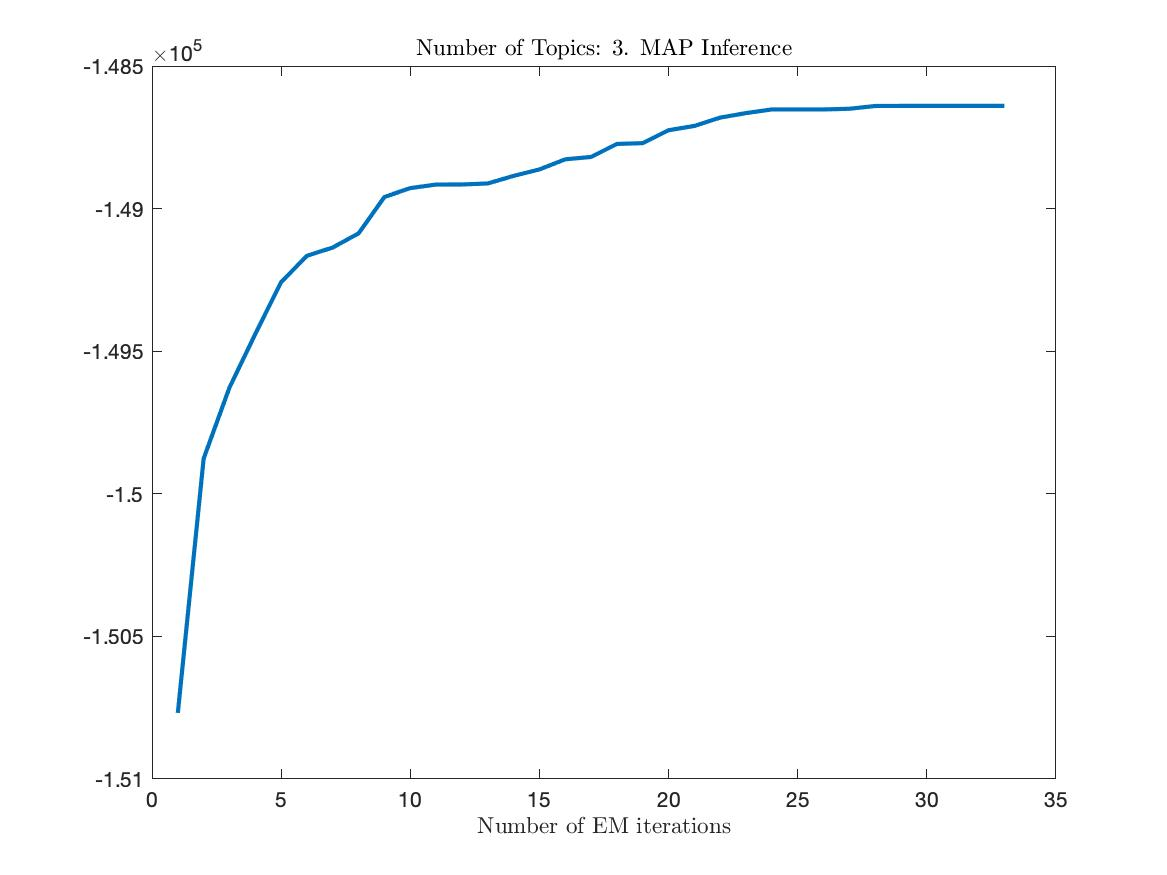
\includegraphics[width=\textwidth]{images/MAP/Q_map_3_topics_alpha11.jpg}
		\caption{}
		\label{fig:Q_MAP_1.1}
	\end{subfigure}
	~	
	\begin{subfigure}{0.4\textwidth}
		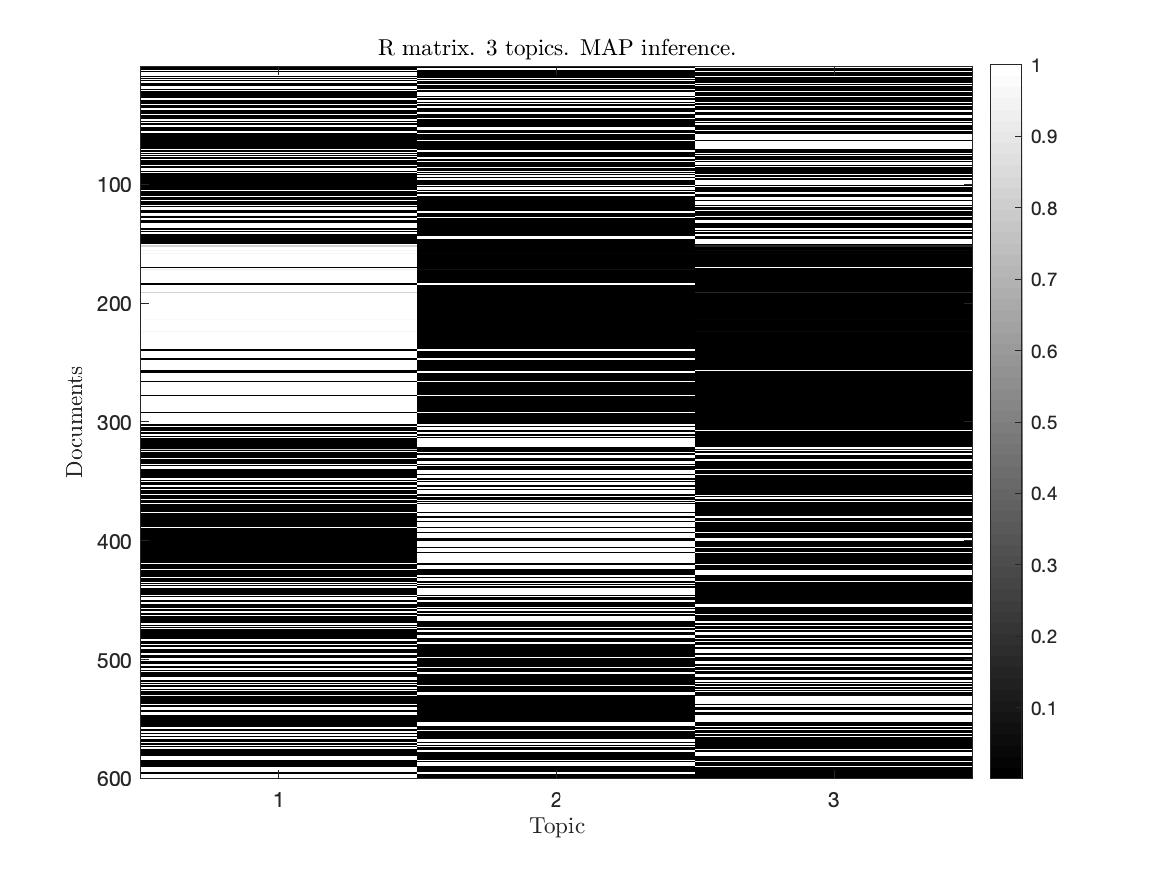
\includegraphics[width=\textwidth]{images/MAP/R_map_3_topics_alpha11.jpg}
		\caption{}
		\label{fig:R_MAP_1.1}
	\end{subfigure}
	\caption{The increase in the posterior in Figure  \ref{fig:Q_MAP_1.1} is not as fast as the ML approach. In Figure \ref{fig:R_MAP_1.1} it can bee seen that thanks to the prior information the different segments of documents are starting to appear.}
	\label{fig:MAP_1.1}
\end{figure}

\subsubsection{Experiment 2: $\bsalpha = 5\I_{Ix1}$}

Now, instead of using a rather uniform distribution for the hyperparameters of the prior we choose a more concentrated distribution by selecting  $\bsalpha = 5\I_{Ix1}$. However, the results are not good as it can be seen in Figure \ref{fig:MAP_5al}. Although the posterior is increasing quite smoothly, when we check the responsibilities $r_{i,k}$ it is clear that the algorithm is just assigning almost all the documents to one topic, and this is clearly not the case. 


% ALPHA = 5
\begin{figure}[h!]
	\centering
	\begin{subfigure}{0.4\textwidth}
		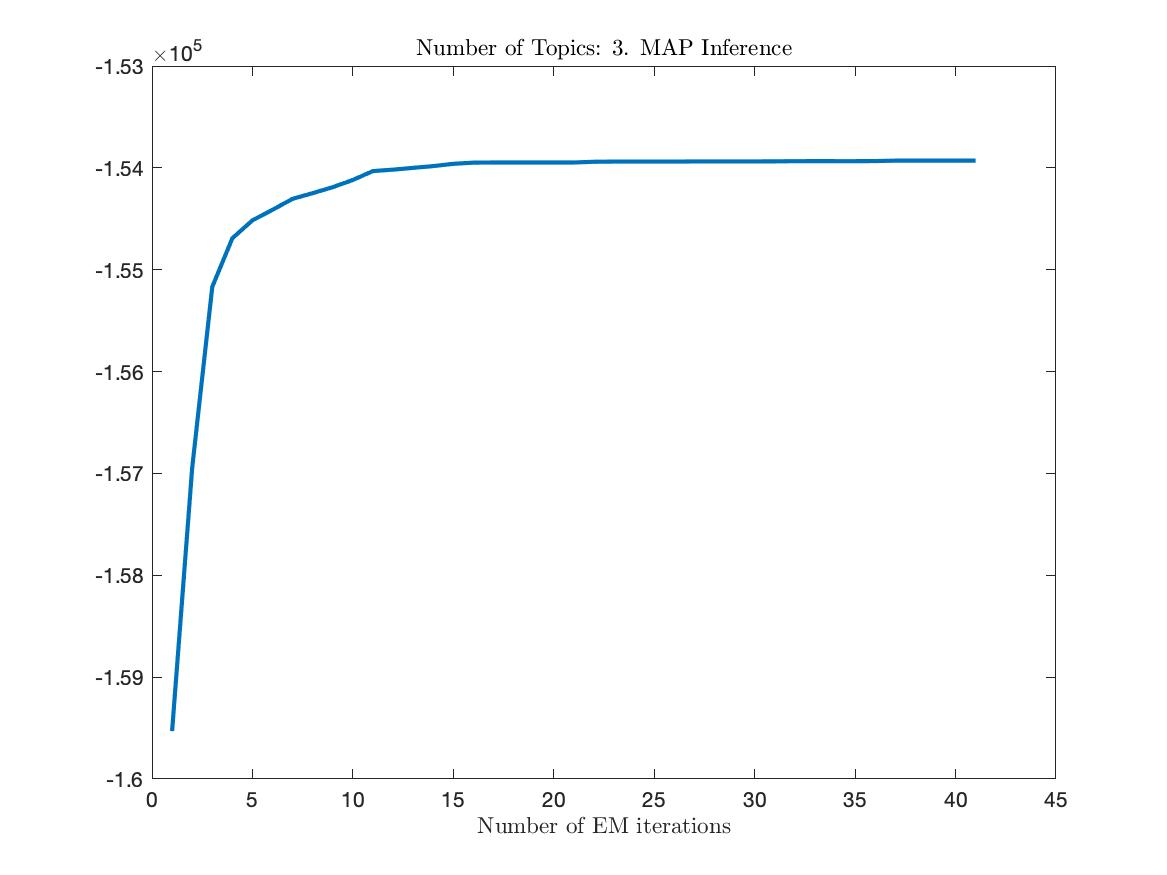
\includegraphics[width=\textwidth]{images/MAP/Q_map_3_topics_alpha5.jpg}
		\caption{}
		\label{fig:Q_MAP_5al}
	\end{subfigure}
	~	
	\begin{subfigure}{0.4\textwidth}
		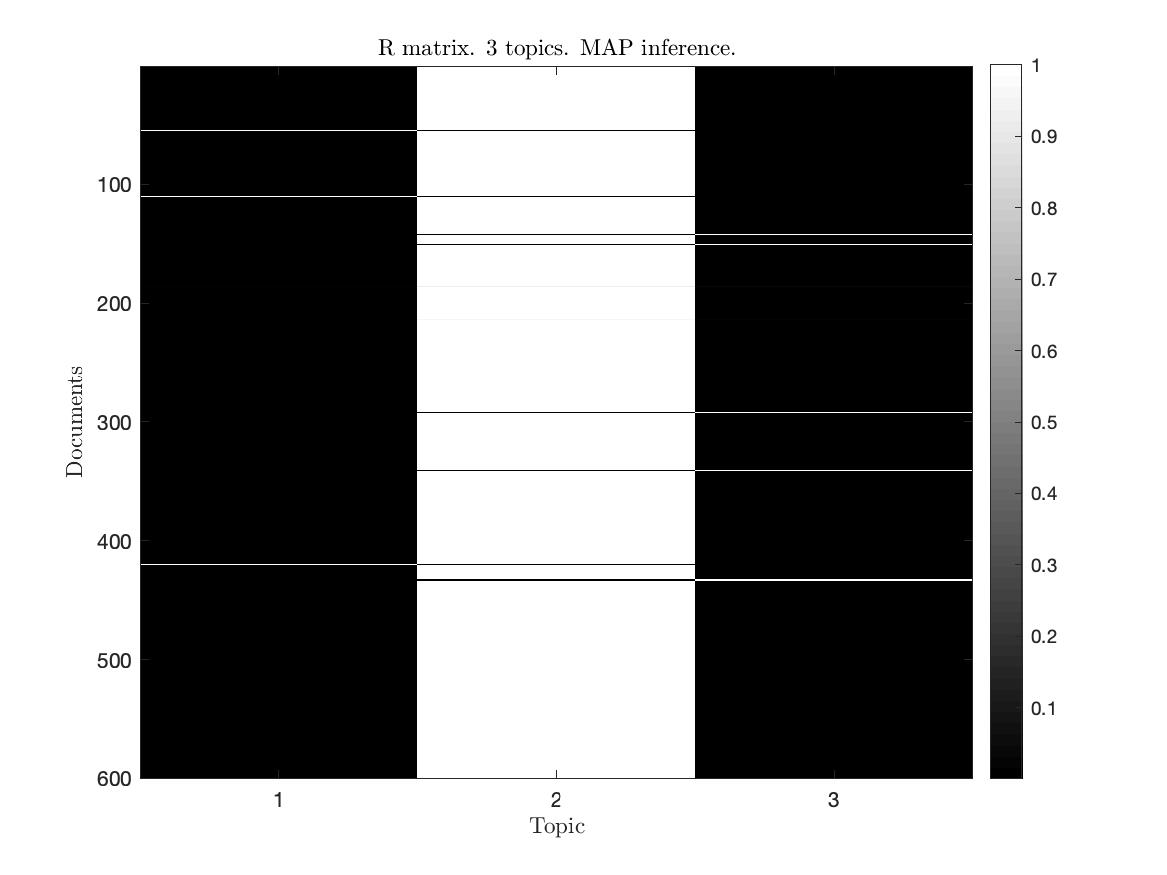
\includegraphics[width=\textwidth]{images/MAP/R_map_3_topics_alpha5.jpg}
		\caption{}
		\label{fig:R_MAP_5al}
	\end{subfigure}
	\caption{Posterior and responsibilities values for the document using $K = 3$ and $\bsalpha = 5\I_{Ix1}$.}
	\label{fig:MAP_5al}
\end{figure}

\subsubsection{Experiment 3: $\bsalpha = 2\I_{Ix1}$}\label{experiment3}

The best solution was actually found for values  $\bsalpha = 2\I_{Ix1}$. In this case the posterior does not increase as fast and smooth as it should, since sometimes some saddle points appear. However, when we check the responsibilities associated to each document, it can be seen that the algorithm is performing rather good. Besides, we will compare the results for different values of $K= 2,3,4,5$.

In Figure \ref{fig:Q_MAP} the different increments of the posterior can be seen. As mentioned above, the increasing for the MAP approach is not as smooth as the ML approach since it depends on the choose of the hyperparameters of the prior. However, the results for the $r_{i,k}$ are quite reasonable, as it can be check in Figure \ref{fig:R_MAP}. For $K=2$ we start to see that the document collection is divided into different segments belonging to the same topic. However, two topics is too general. The best results is found for $K=3$ because we can differentiate three different segments of documents very clearly. For $K=4$ notice that the 4th topic could actually be merged with the first one to form the same topic as in the case with $K=3$. Finally, $K=5$ could be simplified again to three since the 4th topic could be merged with the first topic, and the third topic could be merged with the fifth topic to form $K=3$.


% ALPHA = 2, Q
\begin{figure}[ht]
	\centering
	\begin{subfigure}{0.4\textwidth}
		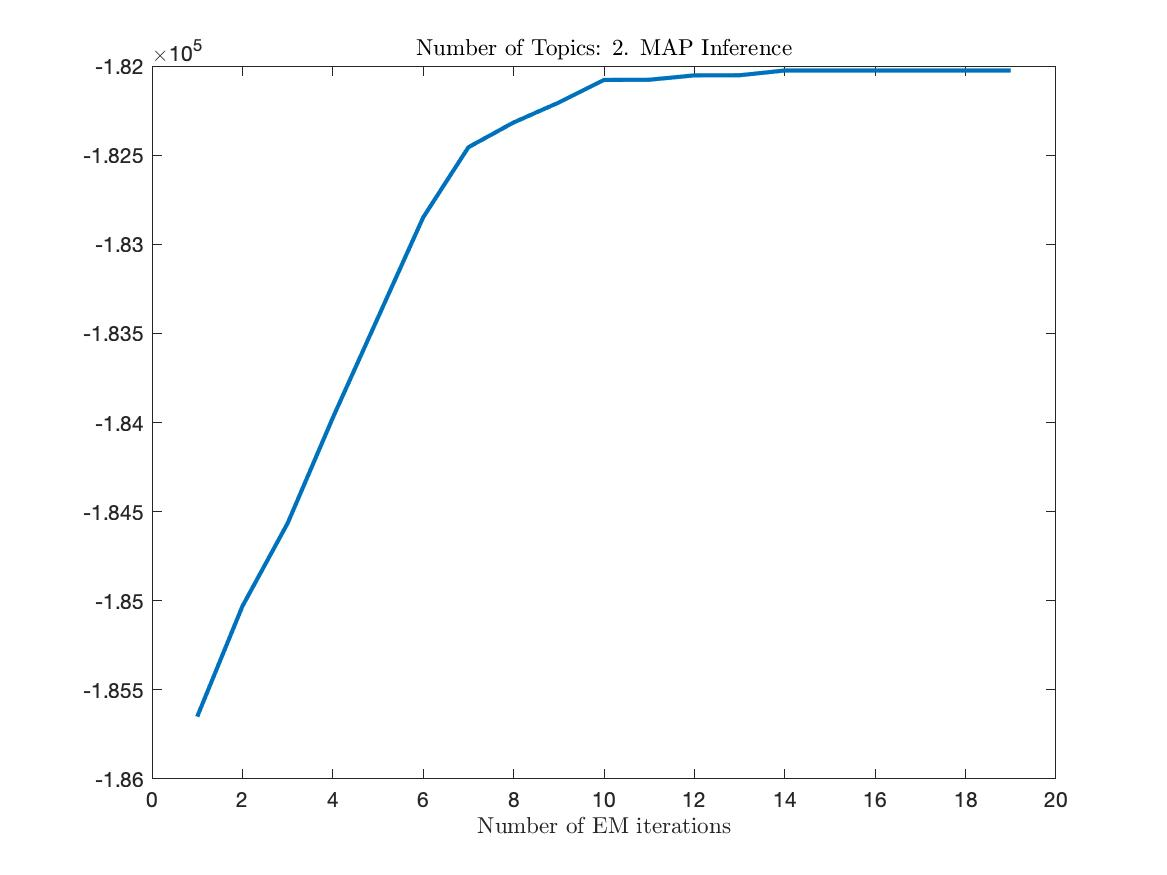
\includegraphics[width=\textwidth]{images/MAP/Q_map_2_topics.jpg}
		\caption{}
		\label{fig:Q_MAP_2}
	\end{subfigure}
	~
	\begin{subfigure}{0.4\textwidth}
		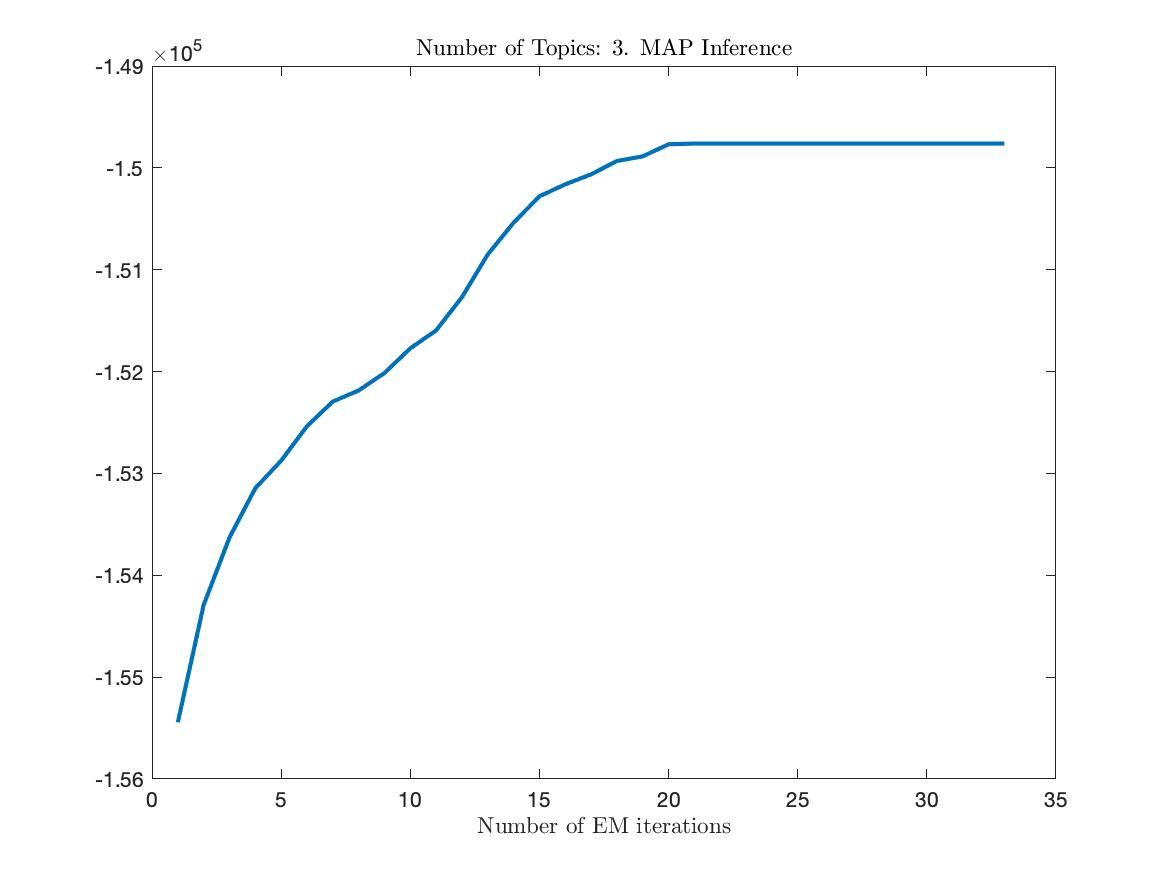
\includegraphics[width=\textwidth]{images/MAP/Q_map_3_topics.jpg}
		\caption{}
		\label{fig:Q_MAP_3}
	\end{subfigure}
	~	
	\begin{subfigure}{0.4\textwidth}
		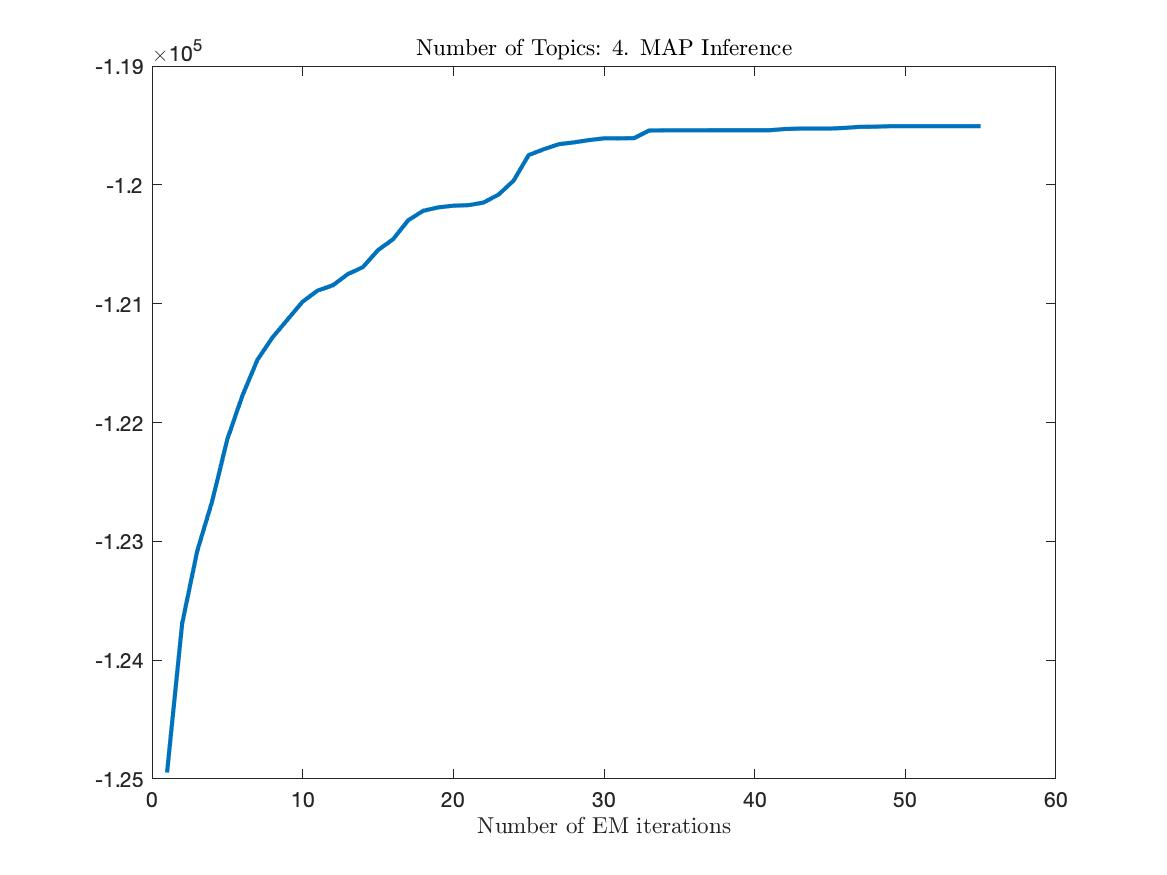
\includegraphics[width=\textwidth]{images/MAP/Q_map_4_topics.jpg}
		\caption{}
		\label{fig:Q_MAP_4}
	\end{subfigure}
	~
	\begin{subfigure}{0.4\textwidth}
	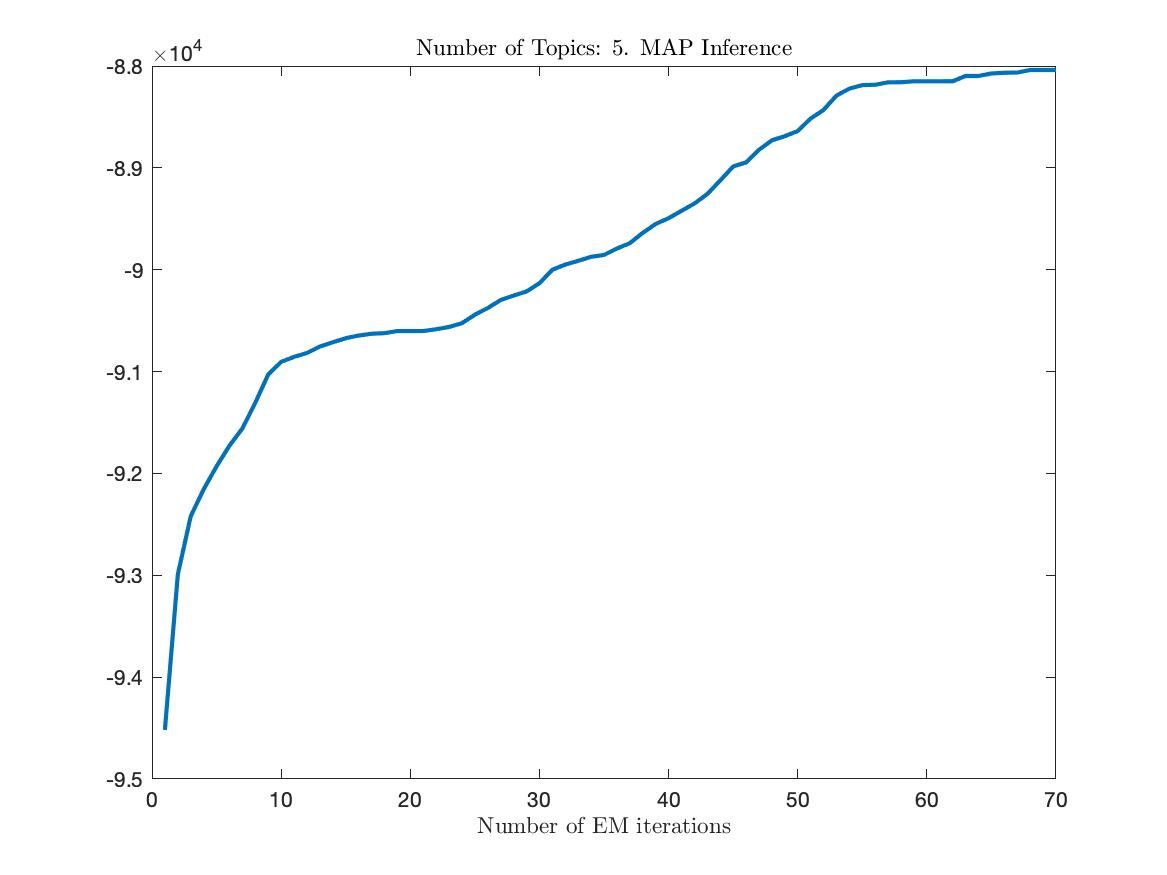
\includegraphics[width=\textwidth]{images/MAP/Q_map_5_topics.jpg}
		\caption{}
		\label{fig:Q_MAP_5}
	\end{subfigure}

	\caption{Increase of the posterior for different values of K.}
	\label{fig:Q_MAP}
\end{figure}

% ALPHA = 2, R
\begin{figure}[hb]
	\centering
	\begin{subfigure}{0.4\textwidth}
		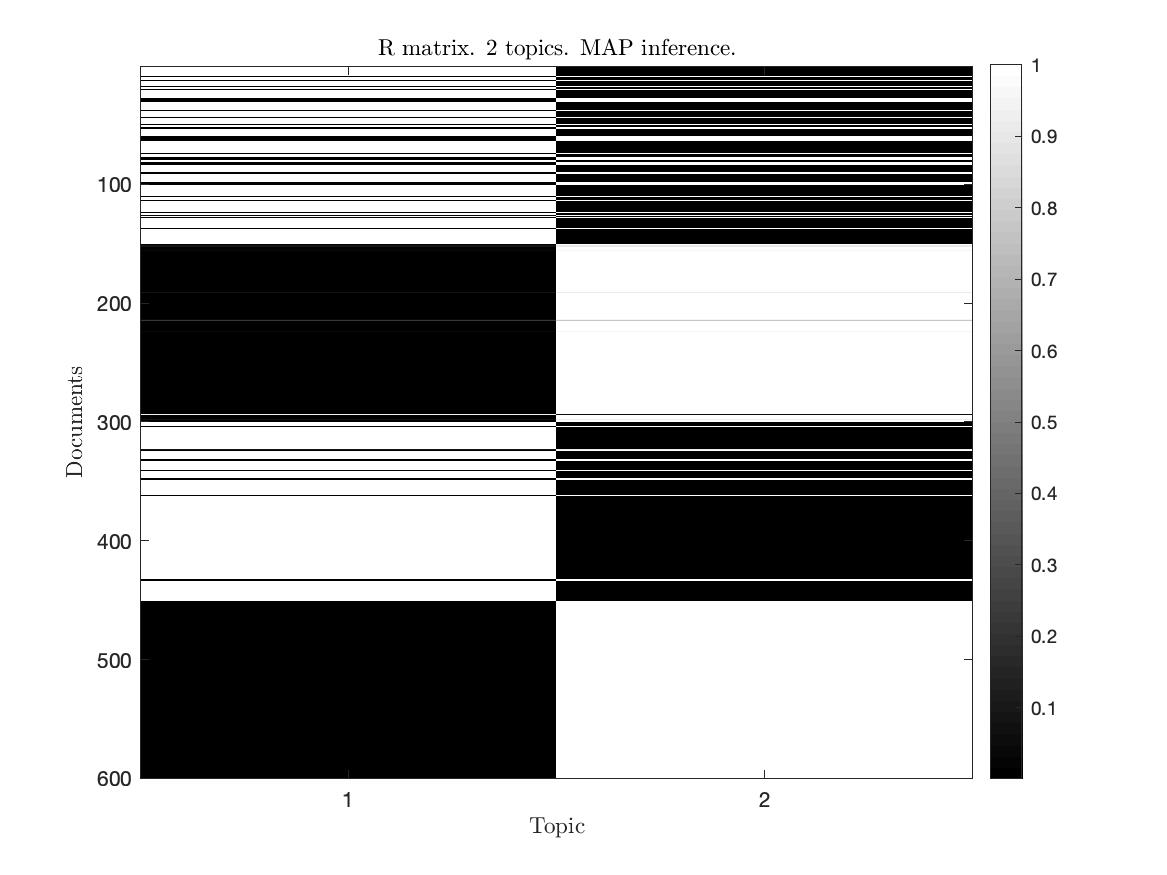
\includegraphics[width=\textwidth]{images/MAP/R_map_2_topics.jpg}
		\caption{}
		\label{fig:R_MAP_2}
	\end{subfigure}
	~
	\begin{subfigure}{0.4\textwidth}
		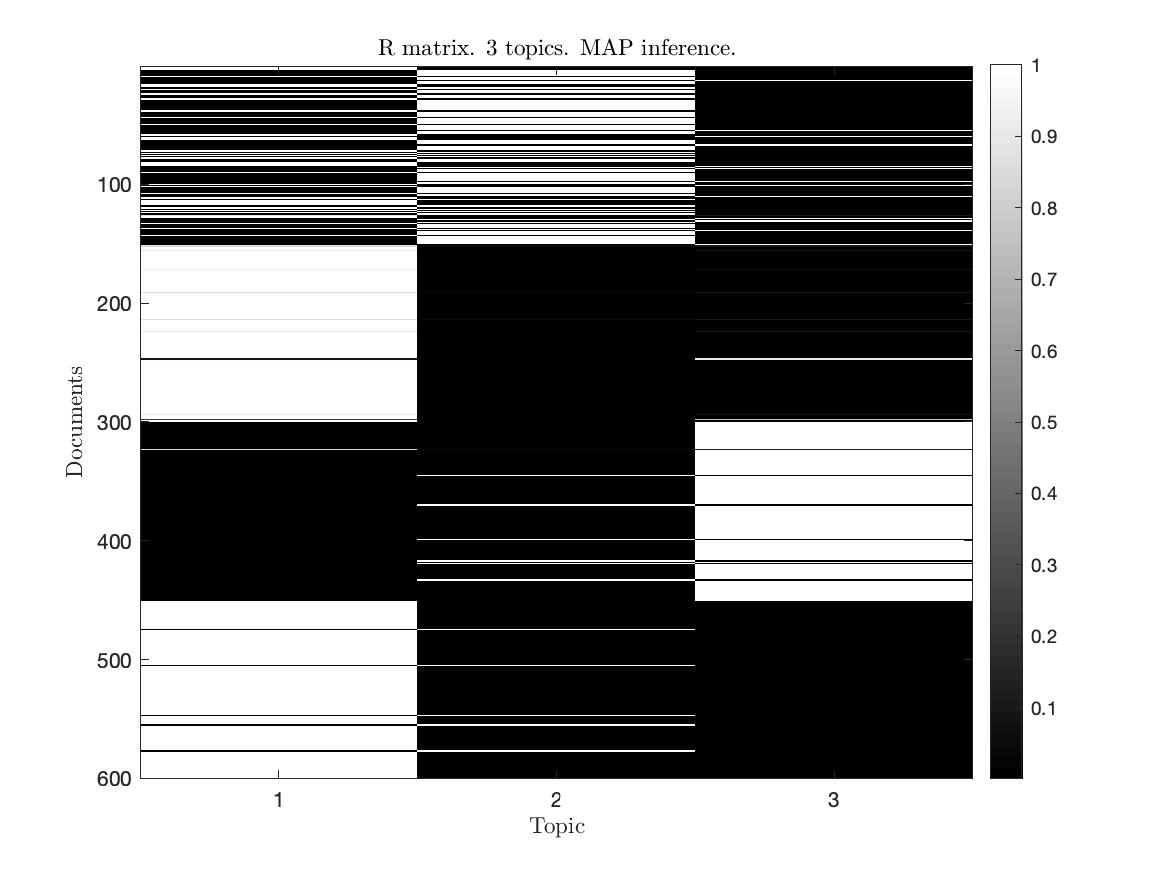
\includegraphics[width=\textwidth]{images/MAP/R_map_3_topics.jpg}
		\caption{}
		\label{fig:R_MAP_3}
	\end{subfigure}
	~	
	\begin{subfigure}{0.4\textwidth}
		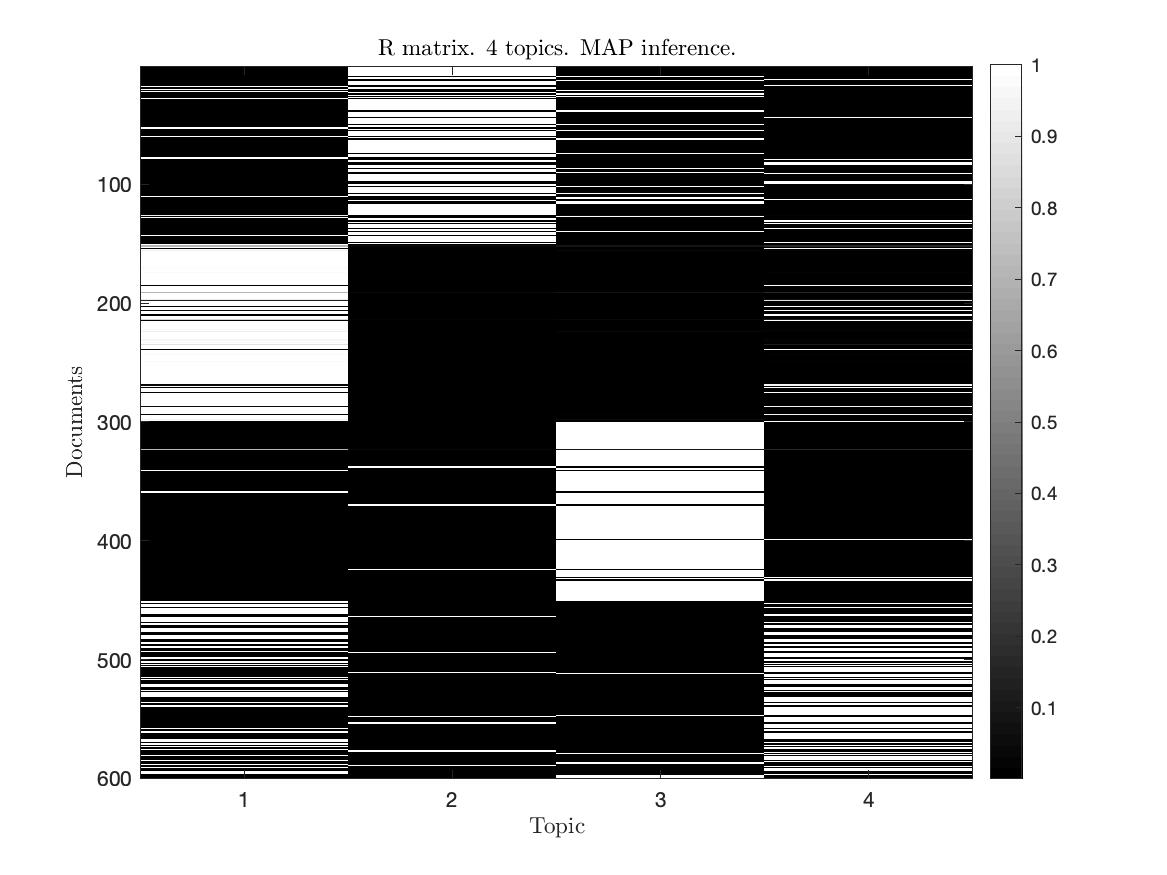
\includegraphics[width=\textwidth]{images/MAP/R_map_4_topics.jpg}
		\caption{}
		\label{fig:R_MAP_4}
	\end{subfigure}
	~
	\begin{subfigure}{0.4\textwidth}
		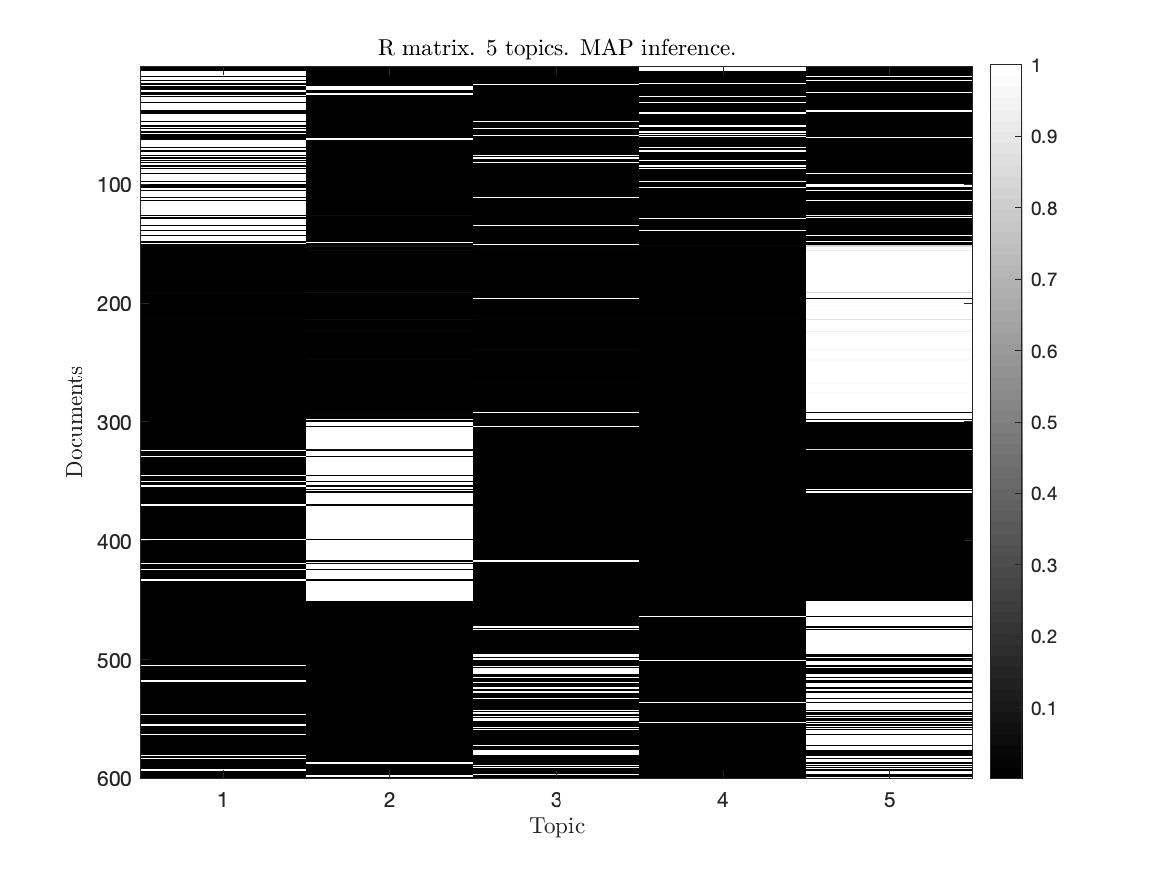
\includegraphics[width=\textwidth]{images/MAP/R_map_5_topics.jpg}
		\caption{}
		\label{fig:R_MAP_5}
	\end{subfigure}
	
	\caption{Responsibilities for each document for different values of K.}
	\label{fig:R_MAP}
\end{figure}

This has been our model selection criterion for selecting $K=3$. At the beginning we tried two Bayesian model criteria, the Bayesian Information Criterion (BIC) and the Akaike Information Criterion (AIC), which are defined with the following formulas

\begin{align}
\mathrm { AIC } & = 2 \text{dof}(\bstheta) - 2 \ln ( \hat { L } )\\
\mathrm { BIC } & = \ln ( n )\text{dof}(\bstheta)- 2 \ln ( \hat { L } ), 
\end{align}
where $ ( \hat { L } )$ is the maximized value of the likelihood function and $\text{dof}(\bstheta)$ is the number of parameters or degrees of freedom of the model. In our case, the number of parameters of the model is 
\begin{equation}
\text{dof}(\bstheta) = K(I-1) + (K-1) = KI-1,
\end{equation}
given by $\bstheta$ and $\bspi$. Since the number of parameters increases with $K$, and the likelihood does not increase that much for different $K$, both criteria were always increasing, and therefore we did not use them to choose the optimal value of $K$. This is illustrated in Figure \ref{fig:ll_bic} where we can see that for increasing number of topics $K$ the log-likelihood always increase and so does the BIC.

\begin{figure}[h]
	\centering
	\begin{subfigure}{0.4\textwidth}
		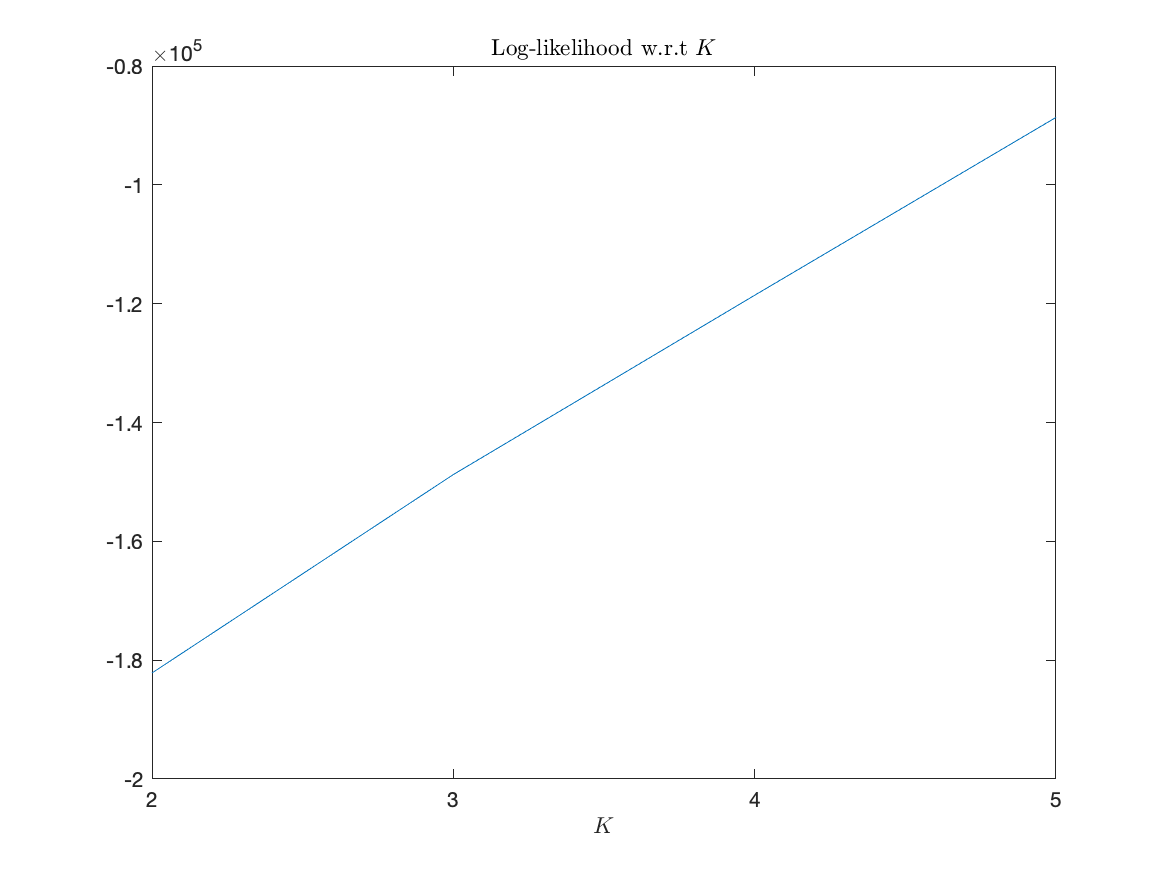
\includegraphics[width=\textwidth]{images/MAP/ll_MAP.png}
		\caption{}
		\label{fig:ll_MAP}
	\end{subfigure}
	~	
	\begin{subfigure}{0.4\textwidth}
		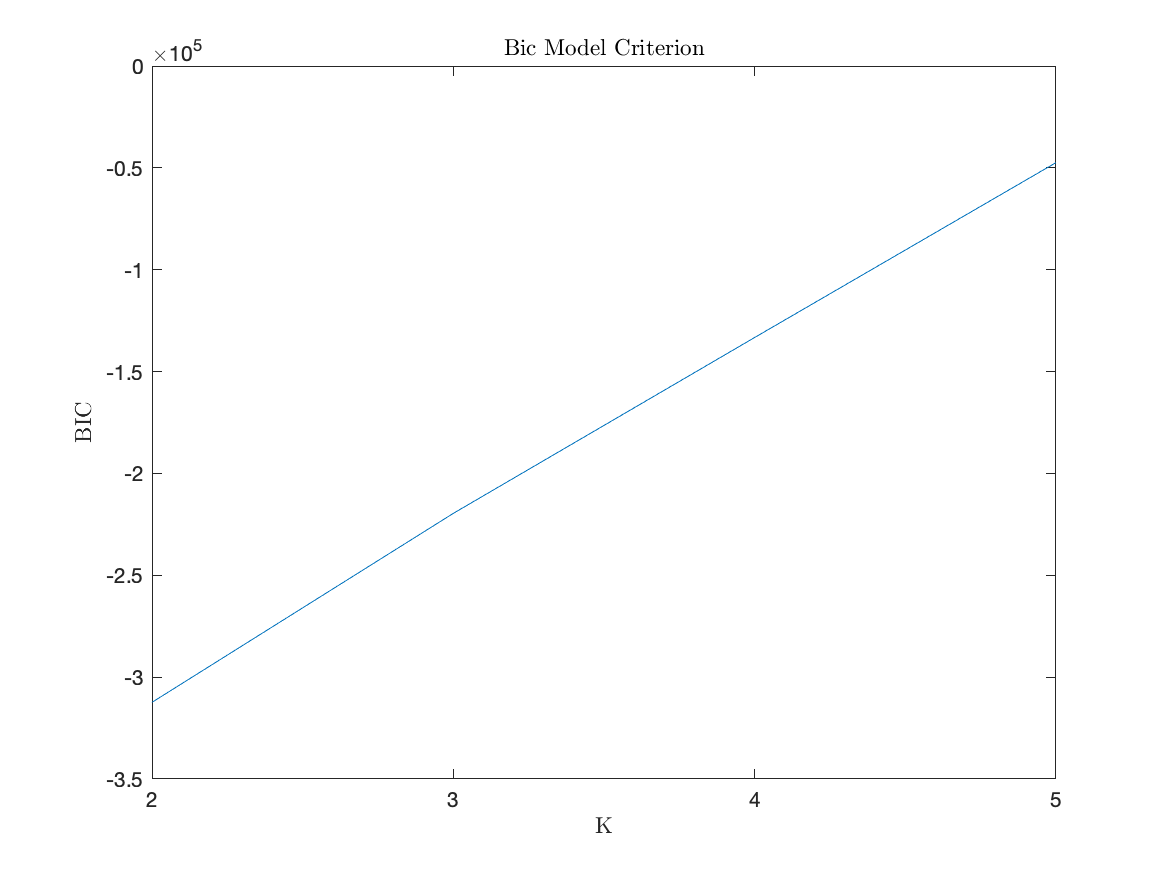
\includegraphics[width=\textwidth]{images/MAP/BIC_MAP.png}
		\caption{}
		\label{fig:bic}
	\end{subfigure}
	\caption{Figure \ref{fig:ll_MAP} shows the log-likelihood increasing for different values of $K$. Figure \ref{fig:bic} shows the BIC model criterion.}
	\label{fig:ll_bic}
\end{figure}


\section{WordCloud visualization}

In order to gain more visual intuition of the solution, we show two Wordclouds generated for Experiment 3 \ref{experiment3} in Figure \ref{fig:clouds}. From the documents belonging to a same topic we obtain the most common word of that certain document so that for each topic we can create a Wordcloud with the most common words per topic. Whit this results it is rather visual to check if a topic is representing a field of research of the provided data.

% WORDCLOUD
\begin{figure}[h]
	\centering
	\begin{subfigure}{0.4\textwidth}
		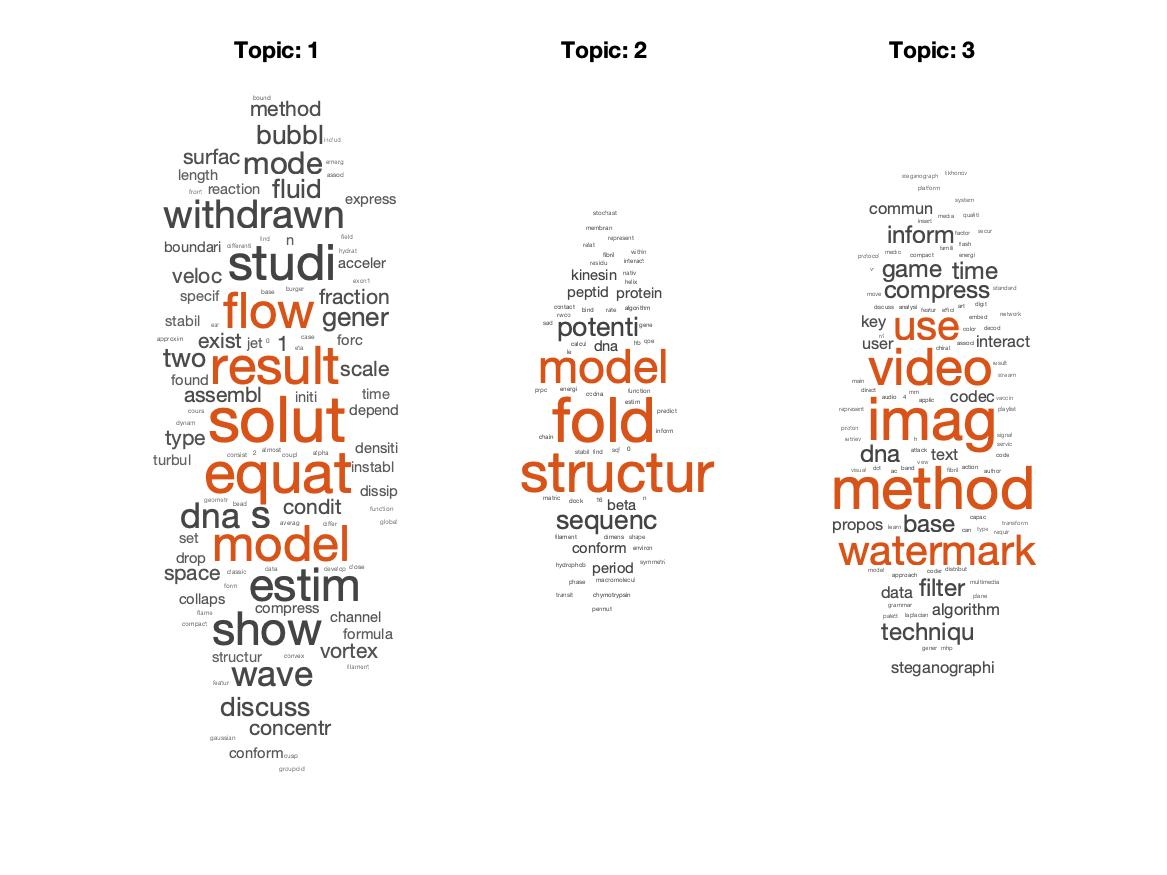
\includegraphics[width=\textwidth]{images/MAP/wordcloud_MAP3_topics.jpg}
		\caption{}
		\label{fig:cloud_3}
	\end{subfigure}
	~	
	\begin{subfigure}{0.4\textwidth}
		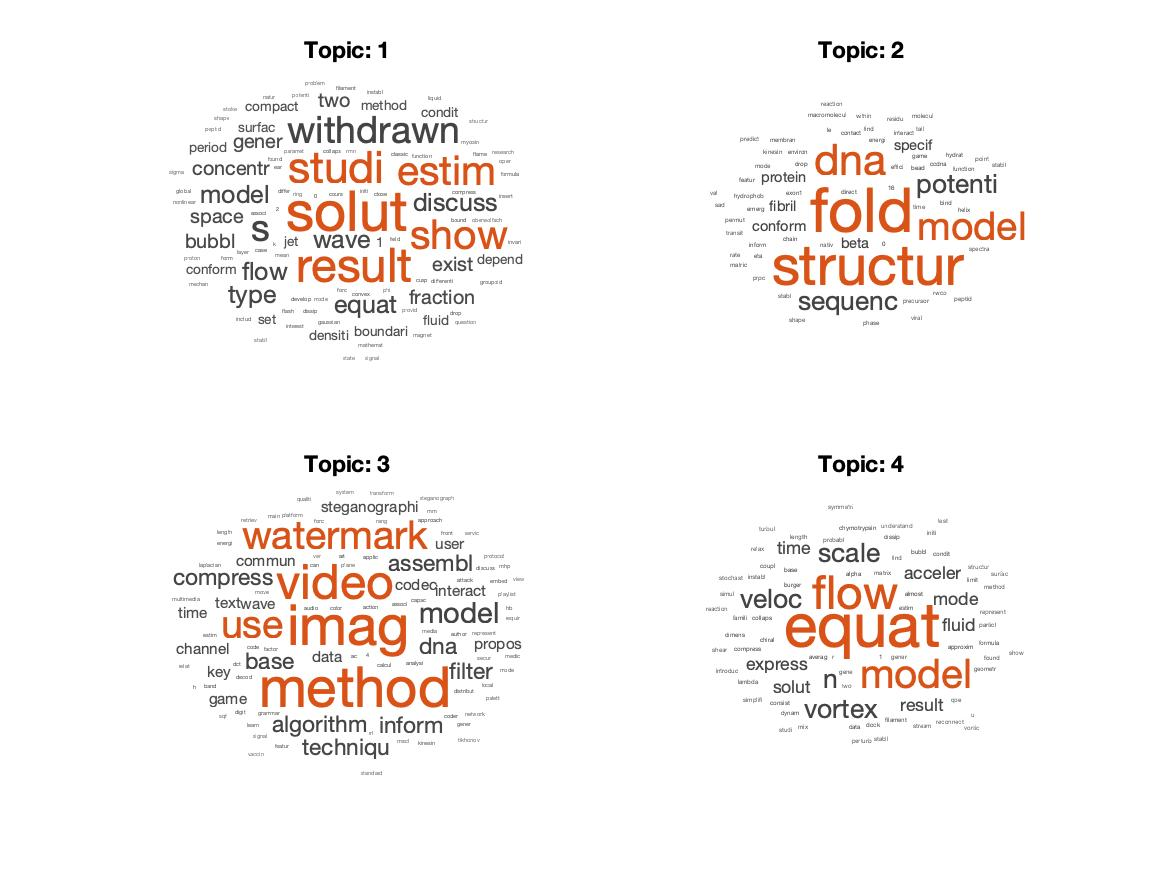
\includegraphics[width=\textwidth]{images/MAP/wordcloud_MAP4_topics.jpg}
		\caption{}
		\label{fig:cloud_4}
	\end{subfigure}
	\caption{The most common words in Topic 1 in Figure \ref{fig:cloud_3} are present in both Topic 1 and Topic 4 \ref{fig:cloud_4}. Therefore, Topic 1 and 4 could be merged together. Notice that each topic is related to a certain field of research from the abstracts.}
	\label{fig:clouds}
\end{figure}


\section{Conclusions}

Throughout this project we have studied the maximum likelihood and the maximum a posterior approach for the Expectation Maximization algorithm applied to a collection of documents following a categorical distribution. It has been shown that using a model in which we know some prior information can achieve better performance characteristics and that the number of mixtures is an important hyperparameter that must be selected according to some criterion. In our case, given the big number of parameters of the model and the small change in the likelihoods for different values of $K$ we  could not use model information criteria and therefore we analyzed the corresponding outputs of the model.

\clearpage
\nocite{*}
\printbibliography

\end{document}

